\documentclass[11pt]{scrartcl}
\usepackage{ucs}
\usepackage[utf8x]{inputenc}
\usepackage[T1]{fontenc}
\usepackage[ngerman,english]{babel} %Text in deutscher Sprache
%\usepackage[english]{babel} %Text in deutscher Sprache
\usepackage{amsmath,amssymb,amstext} %Package für mathematische Umgebung
\usepackage{graphicx} %Bilder hinzufügen
%\usepackage[parfill]{parskip} %no indent as package, else put \noindent
\usepackage{caption}
\usepackage{subcaption}
\usepackage{float}
\usepackage{longtable}
\usepackage{fixltx2e}
\usepackage{textcomp}
\bibliographystyle{habbrv}
 
% itemize in coloumns 
\usepackage{etoolbox,refcount}
\usepackage{multicol}

\newcounter{countitems}
\newcounter{nextitemizecount}
\newcommand{\setupcountitems}{%
  \stepcounter{nextitemizecount}%
  \setcounter{countitems}{0}%
  \preto\item{\stepcounter{countitems}}%
}
\makeatletter
\newcommand{\computecountitems}{%
  \edef\@currentlabel{\number\c@countitems}%
  \label{countitems@\number\numexpr\value{nextitemizecount}-1\relax}%
}
\newcommand{\nextitemizecount}{%
  \getrefnumber{countitems@\number\c@nextitemizecount}%
}
\newcommand{\previtemizecount}{%
  \getrefnumber{countitems@\number\numexpr\value{nextitemizecount}-1\relax}%
}
\makeatother    
\newenvironment{AutoMultiColItemize}{%
\ifnumcomp{\nextitemizecount}{>}{3}{\begin{multicols}{2}}{}%
\setupcountitems\begin{itemize}}%
{\end{itemize}%
\unskip\computecountitems\ifnumcomp{\previtemizecount}{>}{3}{\end{multicols}}{}}


\usepackage{hyperref}
\usepackage{xcolor}
\hypersetup{
    colorlinks,
    linkcolor={black!50!black},
    citecolor={blue!50!black},
    urlcolor={blue!80!black}
}

\title{Bachelorthesis}
\author{Meikee Pagsinohin}

\begin{document}

\tableofcontents
\newpage

\section{Introduction}

	\subsection{Motivation}
		The goal of this project is the improvement in the distinction process between $t\overline{t}\gamma$ and $t\overline{t}$ events in the signal region. Depending on the success, the results can be further used for other projects, which would improve the simulations and their predictions regarding the Standard Model (SM) and Beyond Standard Model (BSM). 

	\subsection{Approach}
	\label{sec:approach}
		An attempt was perfomed through a multivariate analysis by developing and training models. At the beginning, different variables were analysed and compared, and the most promising were then used for training. The type of models, denoted MVA in the following, used for this project are boosted decision trees (BDT) and mutilayer perceptrons (MLP). The results of the MVAs for three different variable categories were created, then analysed and presented in the course of this project.

\section{Background information}
	\subsection{CMS detector and data}
	The CMS detector (compact muon solenoid) is part of the Large Hadron Collider, a particle accelerator, which was built by the research organisation CERN in Geneva, Switzerland. LHC has a circumference of 27km and is up to 175m deep. Besides CMS, there are other experiments as well, such as ATLAS, ALICE and LHCb. CMS has multiple sub-detectors, which all surround the location, where the particles are accelerated and collided against each other.
	
	In Figure \ref{fig:detectorsystem}, a sketch of the detector system can be seen. The inner tracking system is based on silicon detector technology (SI microstrip and pixel) and is used to track charged particles. It is enclosed by electromagnetic and hadron calorimeters (ECAL, HCAL) utilized to prompt showers. They have a barrel and an endcap part and additionally a forward calorimeter was installed to further extend the detector's coverage. The ECAL is built out of lead tungstate crystals and the HCAL is made out of brass and scintillator. Special for the CMS detector is the superconducting solenoid, which surrounds the inner detectors and calorimeters. It has a 6m diameter with a magnetic field of 3.8T used to divert the particle trajectory and to measure their momentum. The muon detectors are positioned in the outermost layer since muons may pass all inner layers \cite{TTG, CMS21, CMS08}.
	
	\begin{figure}[H]
	\centering
	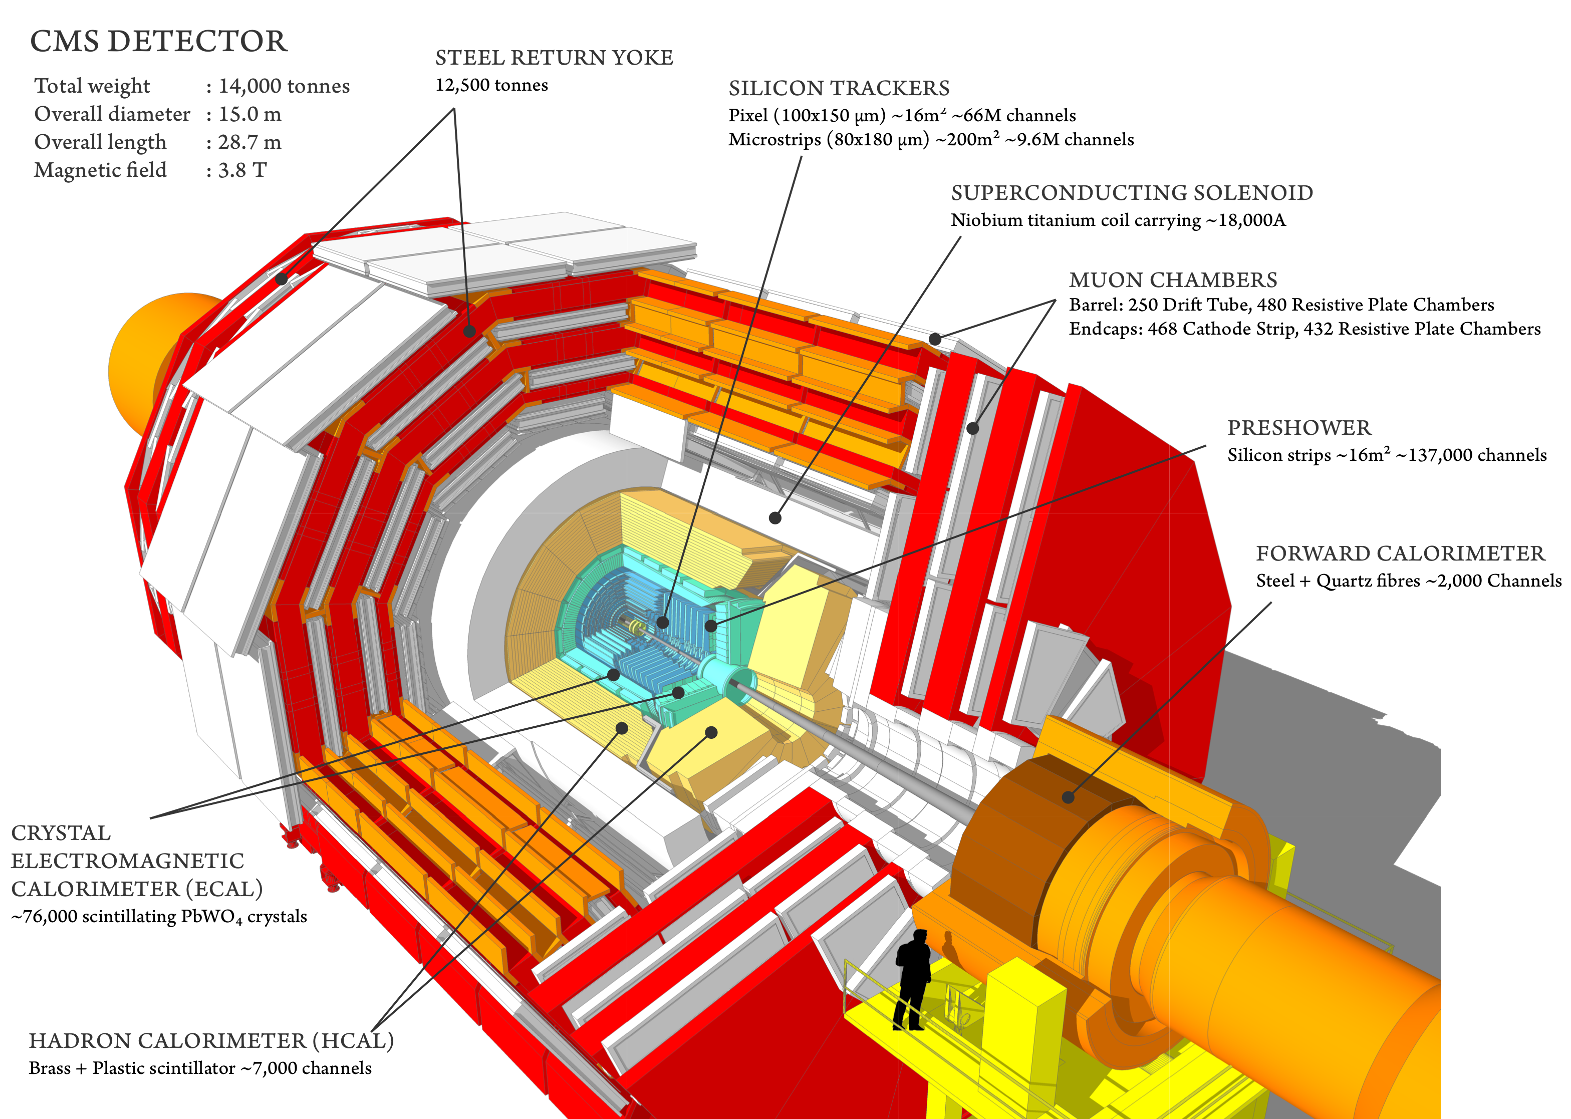
\includegraphics[width=1\textwidth]{figures/detector_system.png}
	\caption{Detector system of CMS}
	\label{fig:detectorsystem}
	\end{figure}
	
	The data is filtered by a two-step trigger system. The hardware-based system (L1) is triggered when muons, electrons, photons and jets with specific characteristics are detected. This reduced the data amount from 40MHz to 100kHz. The software-based system (L2) is triggered by the different energies, type and numbers of particles:
	
\begin{itemize}
  \item lepton has 30/35 GeV
  \item at least 3 jets were detected
  \item at least one of the jets have a b-tag
  \item exactly one photon
\end{itemize}

This reduced the data amount from 100kHz to 1kHz. The data used during this project was recorded in 2016 at a centre-of-mass energy of 13TeV. The signal and background processes were modelled using multiple Monte Carlo event generators~\cite{CMS21}. 

	\subsection{Proton-Proton-collision and $t\overline{t}\gamma$}
	 \label{sec:PPprocess}
	The protons are accelerated in bunches, each containing 10$^{11}$ particles, through different beam pipes in opposite directions and then collided with each other. During the pp collision a top quark pair is produced. The top quark then decays to a W-boson and a b-quark. The W-boson disintegrates into a charged lepton and a corresponding neutrino or a pair of up-type quark and down-type antiquark. The remaining quarks decomposes into jets. This process can be seen in Figure \ref{fig:PPprocess}.
	
	The $t\overline{t}\gamma$ events were selected for this project - top quark pair events with additional photons. The top quark is the heaviest quark in the known elementary particles and is the only quark so far whose properties can be analysed since their lifetime is very short and it forms no bound state before it decays. By that, the electromagnetic coupling, therefore the number of radiated photons after interaction with other charged particles, can be measured~\cite{TTG}. By analysing the top quark, the results can be used to test the Standard Model and its possible extensions~\cite{ATLAS}.
	
	\begin{figure}[H]
	\centering
	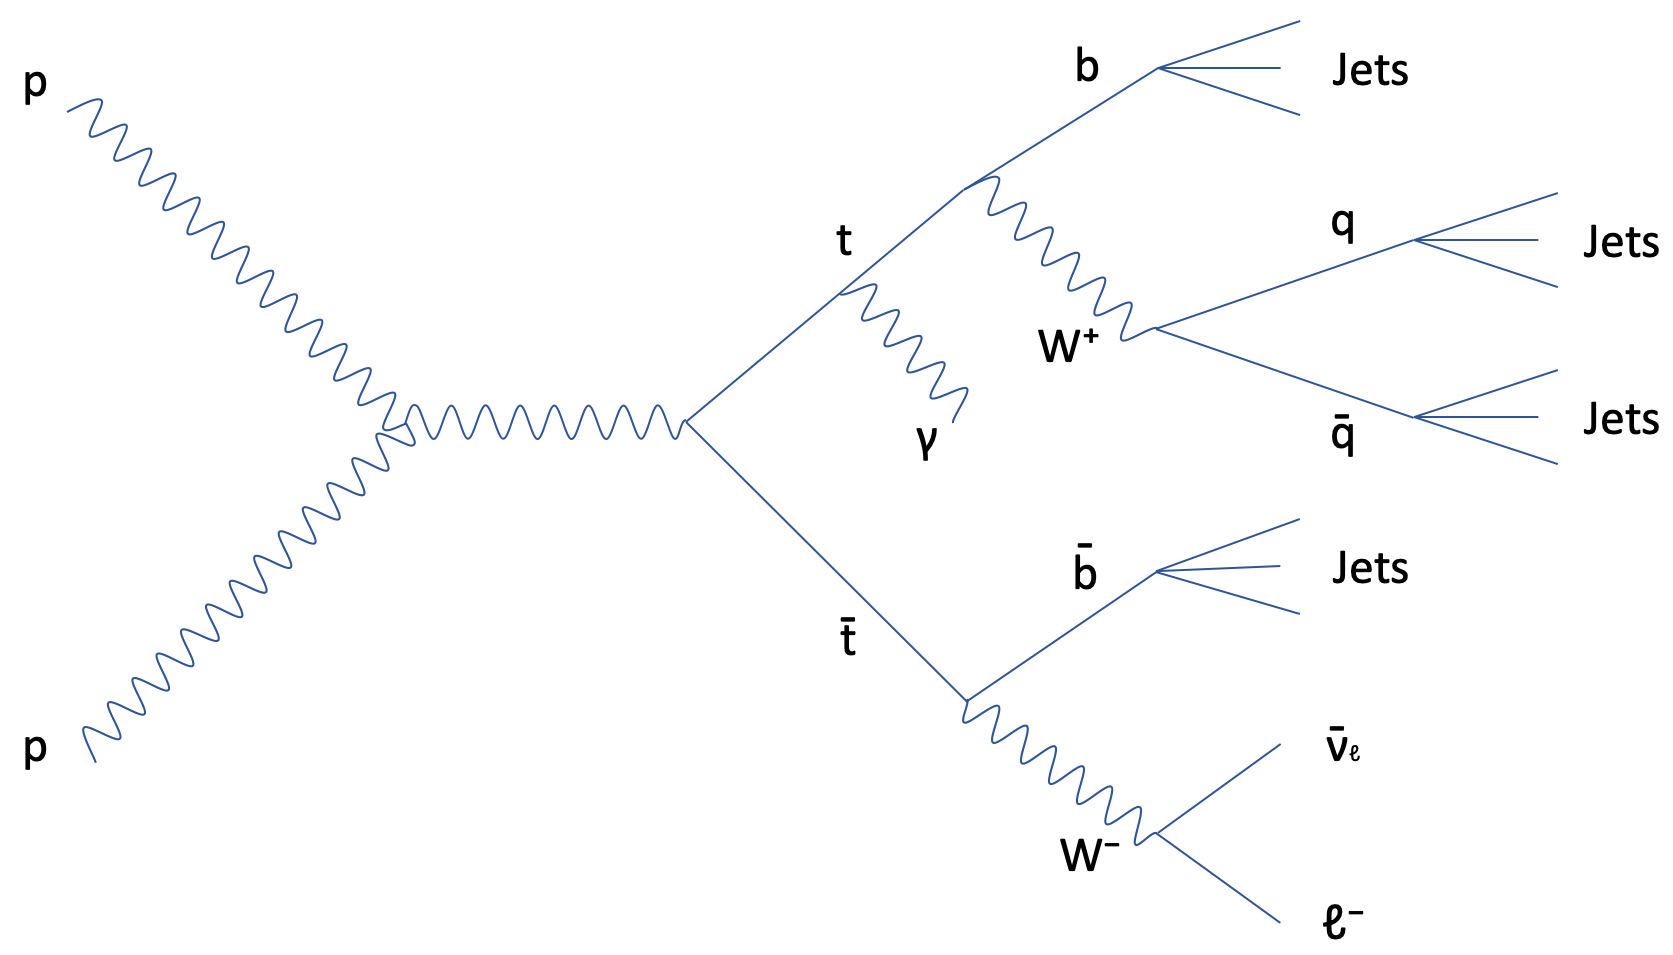
\includegraphics[width=0.9\textwidth]{figures/PP_process.png}
	\caption{Proton Proton collision process}
 	\label{fig:PPprocess}
	\end{figure}
	
\section{Challenge in categorisation}

In Figure \ref{fig:PhotonPT}, the transverse momentum of the photon is visible. The background makes up nearly 50\% of the signal region. The possible sources are~\cite{TTG, ATLAS}:
\begin{itemize}
  \item hadron or electron misidentified as photon
  \item misconstructed photon
  \item photon radiated from different process
  \item additional particles not detected due to limited detector's acceptence
  \item hadron misconstructed as electron
\end{itemize}

A neural network was developed to differentiate between the correctly reconstructed and the misidentified photons. What still needs to be investigated is the possibility of improvement in the discrimination between $t\overline{t}\gamma$ and $t\overline{t}$ events in the signal region through MVAs.

\begin{figure}[H]
\centering
\begin{minipage}{.5\textwidth}
  \centering
  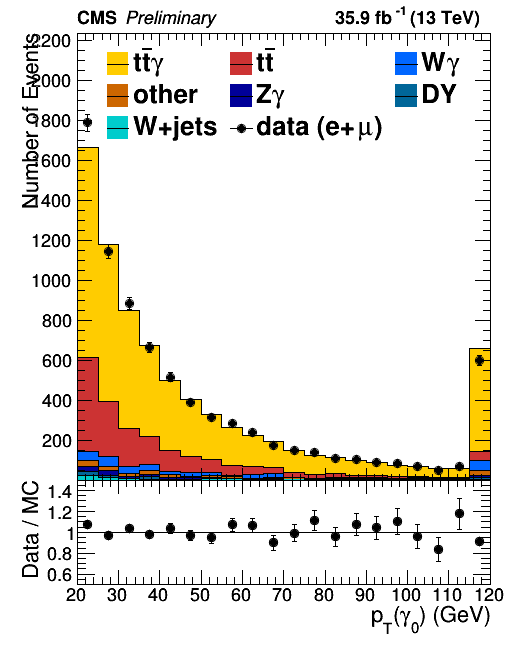
\includegraphics[width=1\linewidth]{figures/PhotonGood0_pt_lin.png}
  \captionof{figure}{Distribution of p\textsubscript{T} photon}
  \label{fig:PhotonPT}
\end{minipage}%
\begin{minipage}{.5\textwidth}
  \centering
  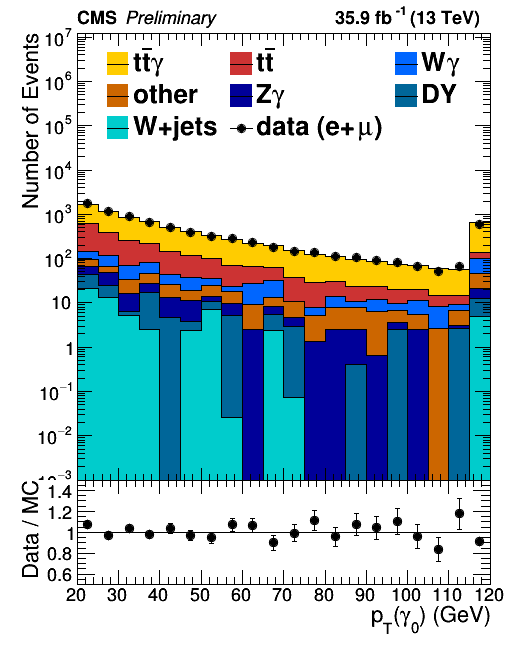
\includegraphics[width=1\linewidth]{figures/PhotonGood0_pt_log.png}
  \captionof{figure}{Distribution of p\textsubscript{T} photon (log)}
  \label{fig:PhotonPTlog}
\end{minipage}
\end{figure}

\section{Analysis process}

	\subsection{Input parameters}
	
The amount of detected particles and the pseudorapidity ($\eta = -ln(tan(\frac{\vartheta}{2}))$, wheras $\vartheta$ is the polar angle) of leptons, photons, first and second jets and b-jets were analysed.  B-jets are jets with a b-tag and the first and second jet refer to the jet with the highest and second highest $p_T$ respectively. The azithmuthal opening angle around the z-axis ($\Delta\phi$) and transverse momentum (p\textsubscript{T}) of these particles were looked at as well. The distance ($\Delta$R = $\sqrt{(\Delta\eta)^2 +(\Delta\phi)^2}$) between lepton and jet, lepton and photon and photon and jet were also considered. 
Additional variables are:
\begin{itemize}
  \item total transverse momentum of all jets; higher amount means either a large number of jets or jets with high energies were detected
  \item maximum mass of three jets; during the decay process of a top quark to a b-quark and W-boson, which further decays to two quarks (see chapter \ref{sec:PPprocess}), the variable would then have a peak at the top quark mass  
  \item transverse mass of an object depending on input variables; if a lepton and neutrino were used in the following formula, then the transverse mass of a W-boson is calculated:
	  \begin{align*}
			m_T(W) = \sqrt{2p_T(\ell)p_T^{miss}[1 - cos(\Delta\phi(\ell, \vec{p}_T^{miss}))]}
		\end{align*}
  
  %\item nPhotonGood0: number of photons
  		\item currently used variable to differentiate between signal and background events
   		\item proportion of energy coming from neutral particles detected in ECAL (e.g. photon)
		\item proportion of energy coming from charged particles detected in ECAL (e.g. electron)
		\item proportion of energy coming from neutral particles detected in HCAL (e.g. neutral meson, neutron)
		\item proportion of energy coming from charged particles detected in HCAL (e.g. charged meson, proton)
  		\item relative isolation of the lepton to all particles in a radius of dR = 0.3 %$\sum_{i} (\frac{p_{T_i}}{p_{T_i}^{LEPTON}})$
		\item relative isolation of the lepton to charged particles in a radius of dR = 0.3 %$\sum_{i} (\frac{p_{T_i}^{CHARGED}}{p_{T_i}^{LEPTON}})$
		\item relative isolation of the lepton to neutral particles in a radius of dR = 0.3 %$\sum_{i} (\frac{p_{T_i}^{NEUTRAL}}{p_{T_i}^{LEPTON}})$
		\item result of neural network to identify first and second jets coming from b-quark (b-tag)
		\item $\Delta\phi$ between lepton and photon
		\item $\Delta\phi$ of missing transverse momentum (MET)
		\item transverse momentum of MET
\end{itemize}

	\subsection{Analysis of variables}
	
The variables were analysed by comparing the distribution of events with a uniform scaling. A uniform scaling was needed to have a better view of relative differences between signal ($t\overline{t}\gamma$) and background ($t\overline{t}$). If the variable shows a different behaviour for each type of event, it could be an indication of discriminatory power. 

Figure \ref{fig:Bj0eta} and \ref{fig:LeptonTight0eta} depict some examples of variables, where the distributions are almost identical and were therefore not analysed any further. A full list of these variables are listed in the Annex, chapter \ref{sec:annex-identical}. 

\begin{figure}[H]
\centering
\begin{minipage}{.5\textwidth}
  \centering
  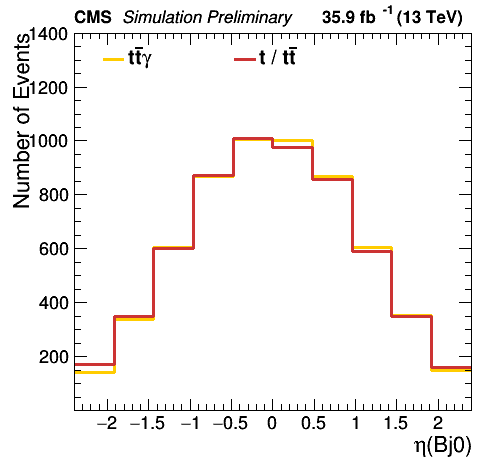
\includegraphics[width=0.70\linewidth]{figures/Notused/Bj0_eta.png}
  %\captionof{figure}{Bj0_eta}
  %\label{fig:Bj0eta}
\end{minipage}%
\begin{minipage}{.5\textwidth}
  \centering
  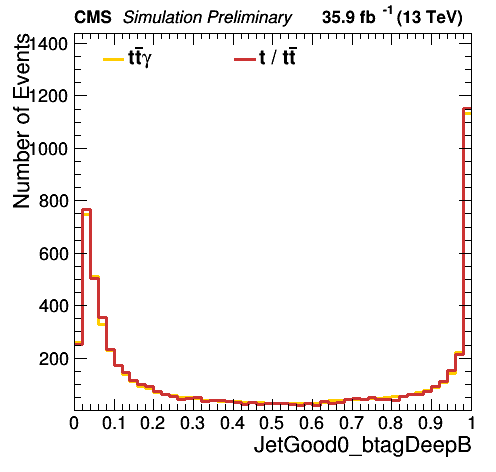
\includegraphics[width=0.70\linewidth]{figures/Notused/JetGood0_btagDeepB.png}
  %\captionof{figure}{JetGood0\_btagDeepB}
  %\label{fig:JetGood0btagDeepB}
\end{minipage}
\captionof{figure}{pseudorapidity of first b-jet and result of neural network to identify b-jets suggest no discriminatory power}
\label{fig:Bj0eta}
\end{figure}

\begin{figure}[H]
\centering
\begin{minipage}{.5\textwidth}
  \centering
  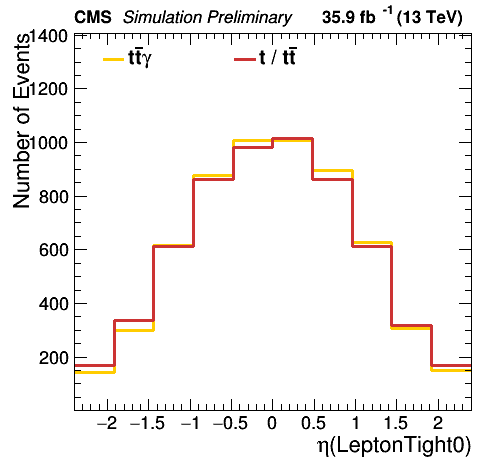
\includegraphics[width=0.70\linewidth]{figures/Notused/LeptonTight0_eta.png}
  %\captionof{figure}{LeptonTight0\_eta}
  %\label{fig:LeptonTight0eta}
\end{minipage}%
\begin{minipage}{.5\textwidth}
  \centering
  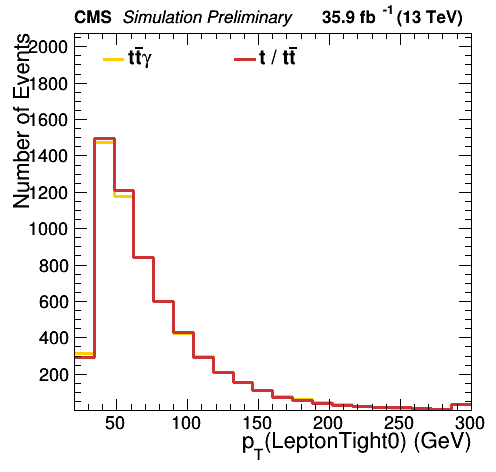
\includegraphics[width=0.70\linewidth]{figures/Notused/LeptonTight0_pt.png}
  %\captionof{figure}{LeptonTight0\_pt}
  %\label{fig:LeptonTight0pt}
\end{minipage}
\captionof{figure}{pseudorapidity and transverse momentum of lepton suggest no discriminatory power}
\label{fig:LeptonTight0eta}
\end{figure}

Variables, where some differences were visible in the signal region, are seen in Figure \ref{fig:nBTagGood} to \ref{fig:ht}. These were candidates for the first set of selected variables. 

	\begin{figure}[H]
	\centering
	\begin{minipage}{.5\textwidth}
	  \centering
	  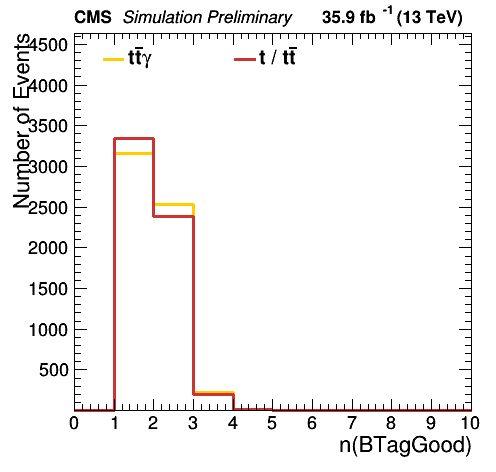
\includegraphics[width=0.70\linewidth]{figures/Select1/nBTagGood.png}
	  %\captionof{figure}{nBTagGood}
	  %\label{fig:nBTagGood}
	\end{minipage}%
	\begin{minipage}{.5\textwidth}
	  \centering
	  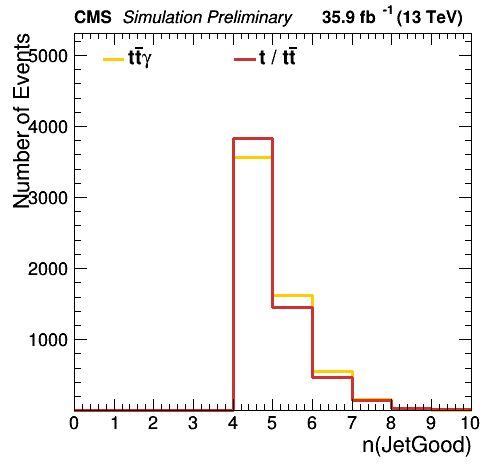
\includegraphics[width=0.70\linewidth]{figures/Select1/nJetGood.png}
	  %\captionof{figure}{nJetGood}
	  %\label{fig:nJetGood}
	\end{minipage}
	\captionof{figure}{number of jets and b-jets show slightly different behaviour between signal and background}
	\label{fig:nBTagGood}
	\end{figure}
	
	\begin{figure}[H]
	\centering
	\begin{minipage}{.5\textwidth}
	  \centering
	  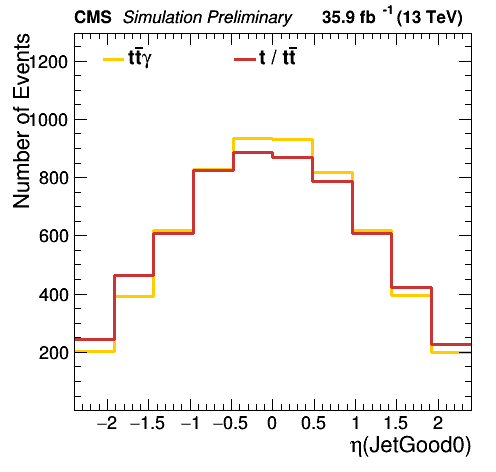
\includegraphics[width=0.70\linewidth]{figures/Select1/JetGood0_eta.png}
	  %\captionof{figure}{JetGood0\_eta}
	  %\label{fig:JetGood0eta}
	\end{minipage}%
	\begin{minipage}{.5\textwidth}
	  \centering
	  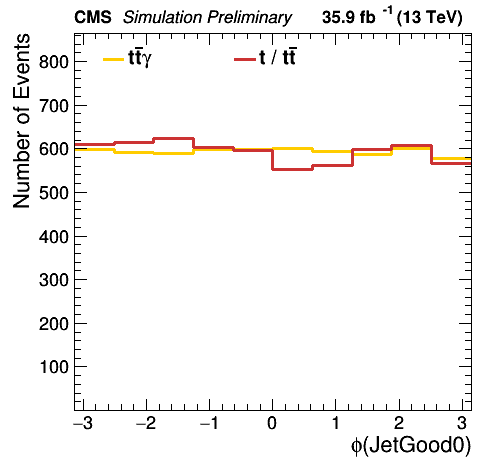
\includegraphics[width=0.70\linewidth]{figures/Select1/JetGood0_phi.png}
	  %\captionof{figure}{JetGood0\_phi}
	  %\label{fig:JetGood0phi}
	\end{minipage}
	\captionof{figure}{pseudorapidity and $\Delta\phi$ of the first jet show slightly different behaviour between signal and background}
	\label{fig:JetGood0phi}
	\end{figure}
	
	\begin{figure}[H]
	\centering
	\begin{minipage}{.5\textwidth}
	  \centering
	  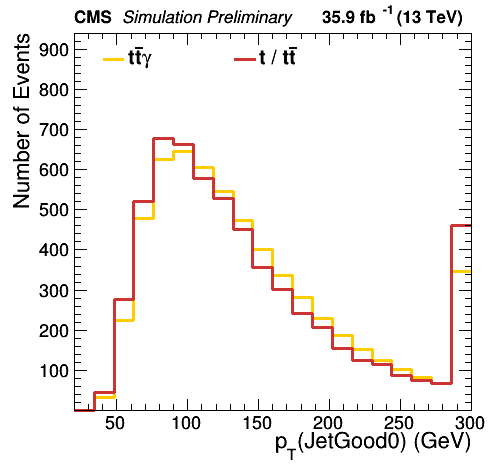
\includegraphics[width=0.70\linewidth]{figures/Select1/JetGood0_pt.png}
	  %\captionof{figure}{JetGood0\_pt}
	  %\label{fig:JetGood0pt}
	\end{minipage}%
	\begin{minipage}{.5\textwidth}
	  \centering
	  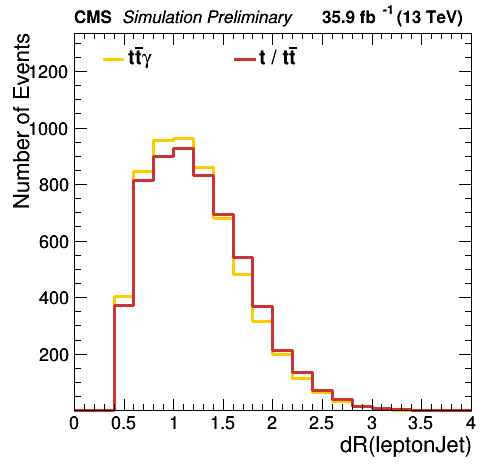
\includegraphics[width=0.70\linewidth]{figures/Select1/leptonJetdR.png}
	  %\captionof{figure}{leptonJetdR}
	  %\label{fig:leptonJetdR}
	\end{minipage}
	\captionof{figure}{transverse momentum of first jet and distance between lepton and jet show slightly different behaviour between signal and background}
	\end{figure}
	
	\begin{figure}[H]
	\centering
	\begin{minipage}{.5\textwidth}
	  \centering
	  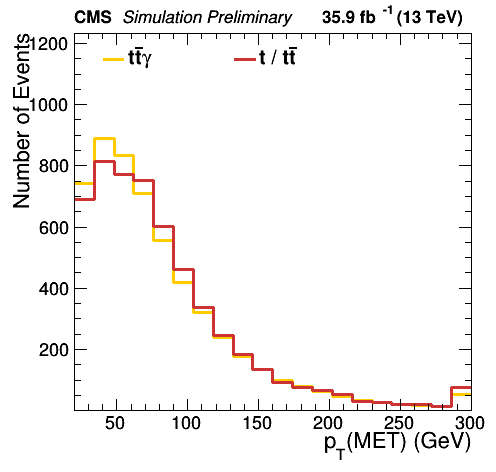
\includegraphics[width=0.70\linewidth]{figures/Select1/MET_pt.png}
	  %\captionof{figure}{MET\_pt}
	  %\label{fig:METpt}
	\end{minipage}%
	\begin{minipage}{.5\textwidth}
	  \centering
	  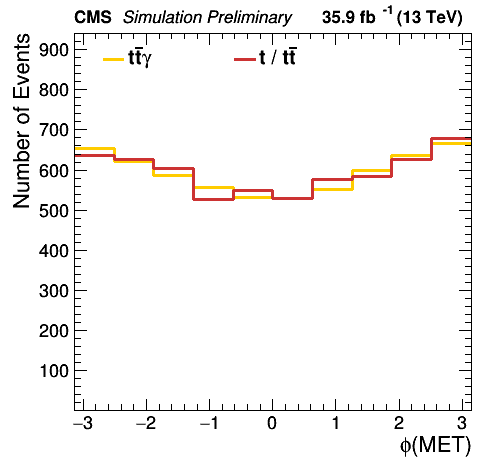
\includegraphics[width=0.70\linewidth]{figures/Select1/MET_phi.png}
	  %\captionof{figure}{MET\_phi}
	  %\label{fig:METphi}
	\end{minipage}
	\captionof{figure}{transverse momentum and $\Delta\phi$ of missing transverse momentum show slightly different behaviour between signal and background}
	\end{figure}
	
	\begin{figure}[H]
	\centering
	\begin{minipage}{.5\textwidth}
	  \centering
	  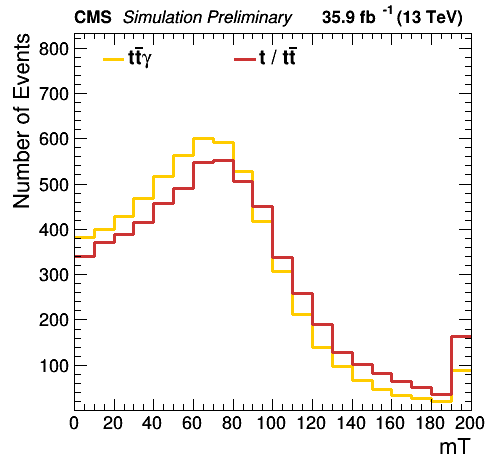
\includegraphics[width=0.70\linewidth]{figures/Select1/mT.png}
	  %\captionof{figure}{mT}
	  %\label{fig:mT}
	\end{minipage}%
	\begin{minipage}{.5\textwidth}
	  \centering
	  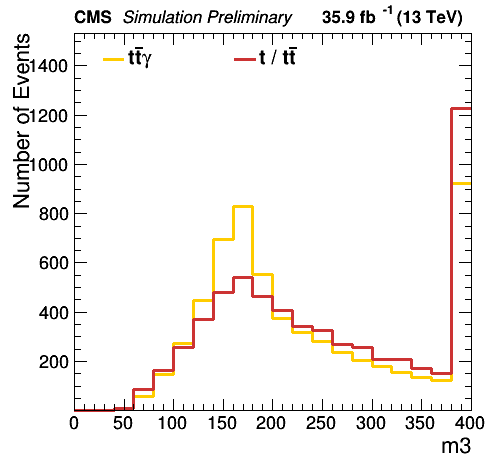
\includegraphics[width=0.70\linewidth]{figures/Select1/m3.png}
	  %\captionof{figure}{m3}
	  %\label{fig:m3}
	\end{minipage}
	\captionof{figure}{transverse momentum of W-boson and maximum mass of three jets show slightly different behaviour between signal and background}
	\end{figure}

	\begin{figure}[H]
	\centering
	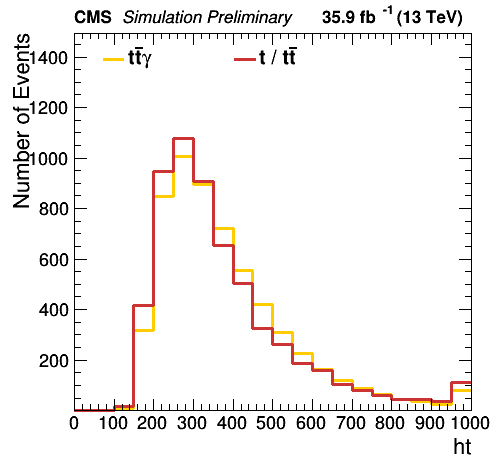
\includegraphics[width=0.35\textwidth]{figures/Select1/ht.png}
	\caption{transverse momentum of all jets show slightly different behaviour between signal and background}
 	\label{fig:ht}
	\end{figure}
	
\newpage
The currently used variable to differentiate between $t\overline{t}\gamma$ and $t\overline{t}$, seen in Figure \ref{fig:PhotonGood0mvaID}, shows quite a good distinction and is therefore added to the list (second selection).

	\begin{figure}[H]
	\centering
	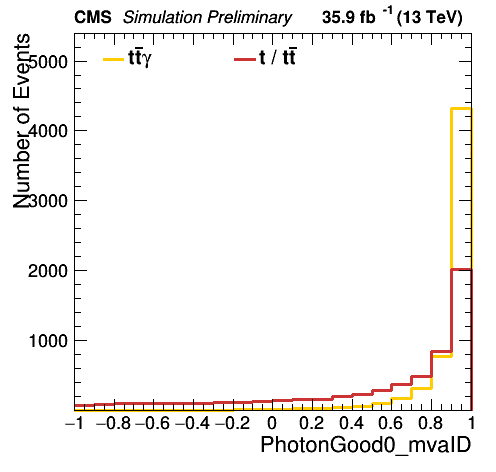
\includegraphics[width=0.35\textwidth]{figures/Select2/PhotonGood0_mvaID.png}
	\caption{currently used variable to differentiate between signal and background events suggests good distinction}
 	\label{fig:PhotonGood0mvaID}
	\end{figure}
	
Figure \ref{fig:PhotonGood0pt} to \ref{fig:photonLepdR} are the photon variables. These demonstrate the most promising behaviour for discriminating between $t\overline{t}\gamma$ and $t\overline{t}$ events and were additionally put into the third selection category.

	\begin{figure}[H]
	\centering
	\begin{minipage}{.5\textwidth}
	  \centering
	  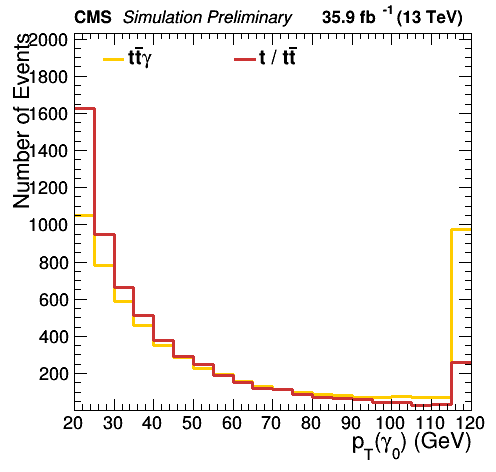
\includegraphics[width=0.70\linewidth]{figures/Select3/PhotonGood0_pt.png}
	  %\captionof{figure}{PhotonGood0\_pt}
	  %\label{fig:PhotonGood0pt}
	\end{minipage}%
	\begin{minipage}{.5\textwidth}
	  \centering
	  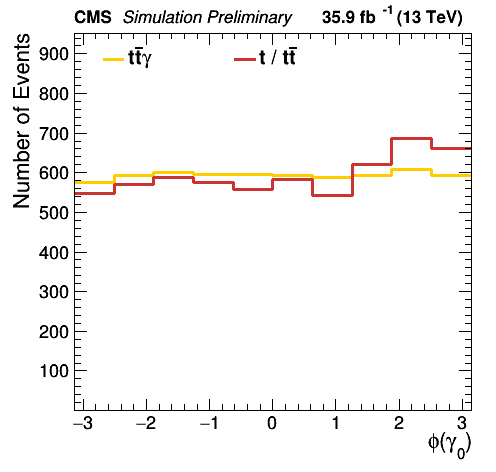
\includegraphics[width=0.70\linewidth]{figures/Select3/PhotonGood0_phi.png}
	  %\captionof{figure}{PhotonGood0\_phi}
	  %\label{fig:PhotonGood0phi}
	\end{minipage}
	\caption{transverse momentum and $\Delta\phi$ of photon indicate good discriminatory power}
	\label{fig:PhotonGood0pt}
	\end{figure}
	
	\begin{figure}[H]
	\centering
	\begin{minipage}{.5\textwidth}
	  \centering
	  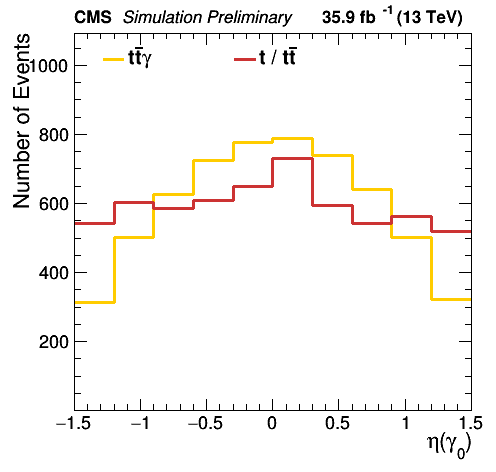
\includegraphics[width=0.70\linewidth]{figures/Select3/PhotonGood0_eta.png}
	  %\captionof{figure}{PhotonGood0\_eta}
	  %\label{fig:PhotonGood0eta}
	\end{minipage}%
	\begin{minipage}{.5\textwidth}
	  \centering
	  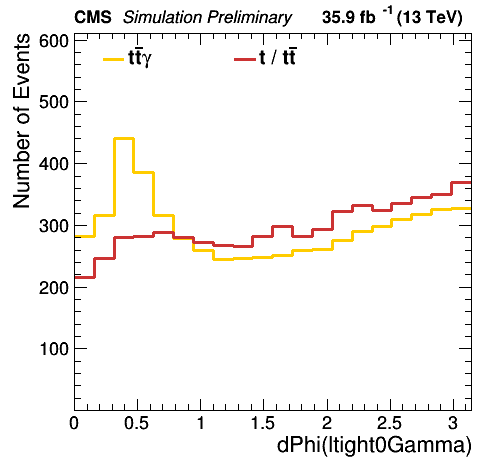
\includegraphics[width=0.70\linewidth]{figures/Select3/ltight0GammadPhi.png}
	  %\captionof{figure}{ltight0GammadPhi}
	  %\label{fig:ltight0GammadPhi}
	\end{minipage}
	\caption{pseudorapidity of photon and $\Delta\phi$ between lepton and photon indicate good discriminatory power}
	\end{figure}
	
	\begin{figure}[H]
	\centering
	\begin{minipage}{.5\textwidth}
	  \centering
	  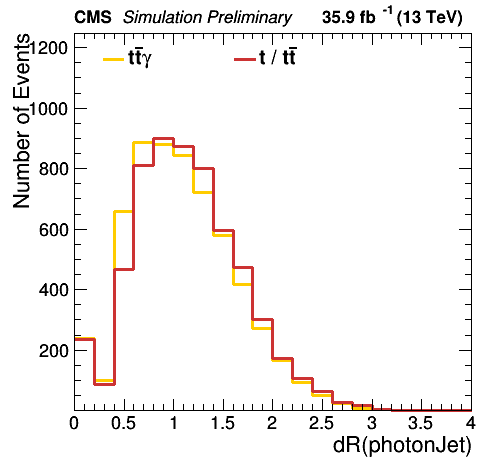
\includegraphics[width=0.70\linewidth]{figures/Select3/photonJetdR.png}
	  %\captionof{figure}{photonJetdR}
	  %\label{fig:photonJetdR}
	\end{minipage}%
	\begin{minipage}{.5\textwidth}
	  \centering
	  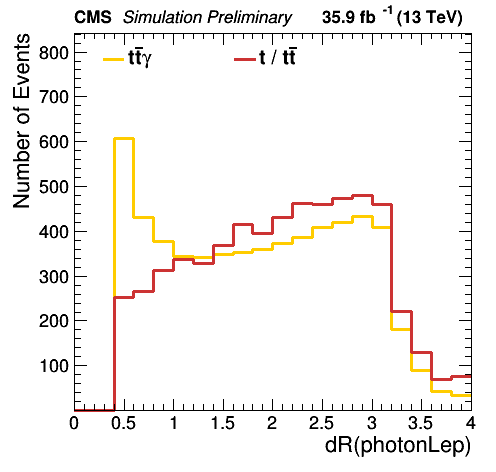
\includegraphics[width=0.70\linewidth]{figures/Select3/photonLepdR.png}
	  %\captionof{figure}{photonLepdR}
	  %\label{fig:photonLepdR}
	\end{minipage}
	\caption{distance between photon and jet and between photon and lepton indicate good discriminatory power}
	\label{fig:photonLepdR}
	\end{figure}

\section{MVA}

Trying to split signal and background through a variable with a cut-off value faces the problem that this criteria doesn't apply for every event. If it works for one event, it doesn't mean that it works for the next one. Therefore, mutliple variables need to be used to distinguish between those two categories, so called multivariate analysis (MVA). As already mentioned in chapter \ref{sec:approach}, the chosen MVA-types are boosted decision trees (BDT) and multilayer perceptron (MLP).

	\subsection{BDT - Boosted Decision Trees}
	The decision tree starts with the root node containing the whole sample. For a binary tree, the node is then split into two branches using a variable and a corresponding cut-off value. The cut-off value should be a value that seperates the signal from the background the best. This process will be repeated for each branch for all relevant variables, including already used variables, until an end criteria is met. The final branch is called a leaf and this will be assigned to one of the two categories. End criterias could be a minimum size of a leaf, perfect separation, insignificant improvement after split or maximal tree depth. Boosted decision trees are built out of additional trees, so called weak classifieres. They include variables with a low discriminatory power and will be used to improve the main decision tree to a more stable model with a lower error rate~\cite{BDT}. 

	\begin{figure}[H]
	\centering
	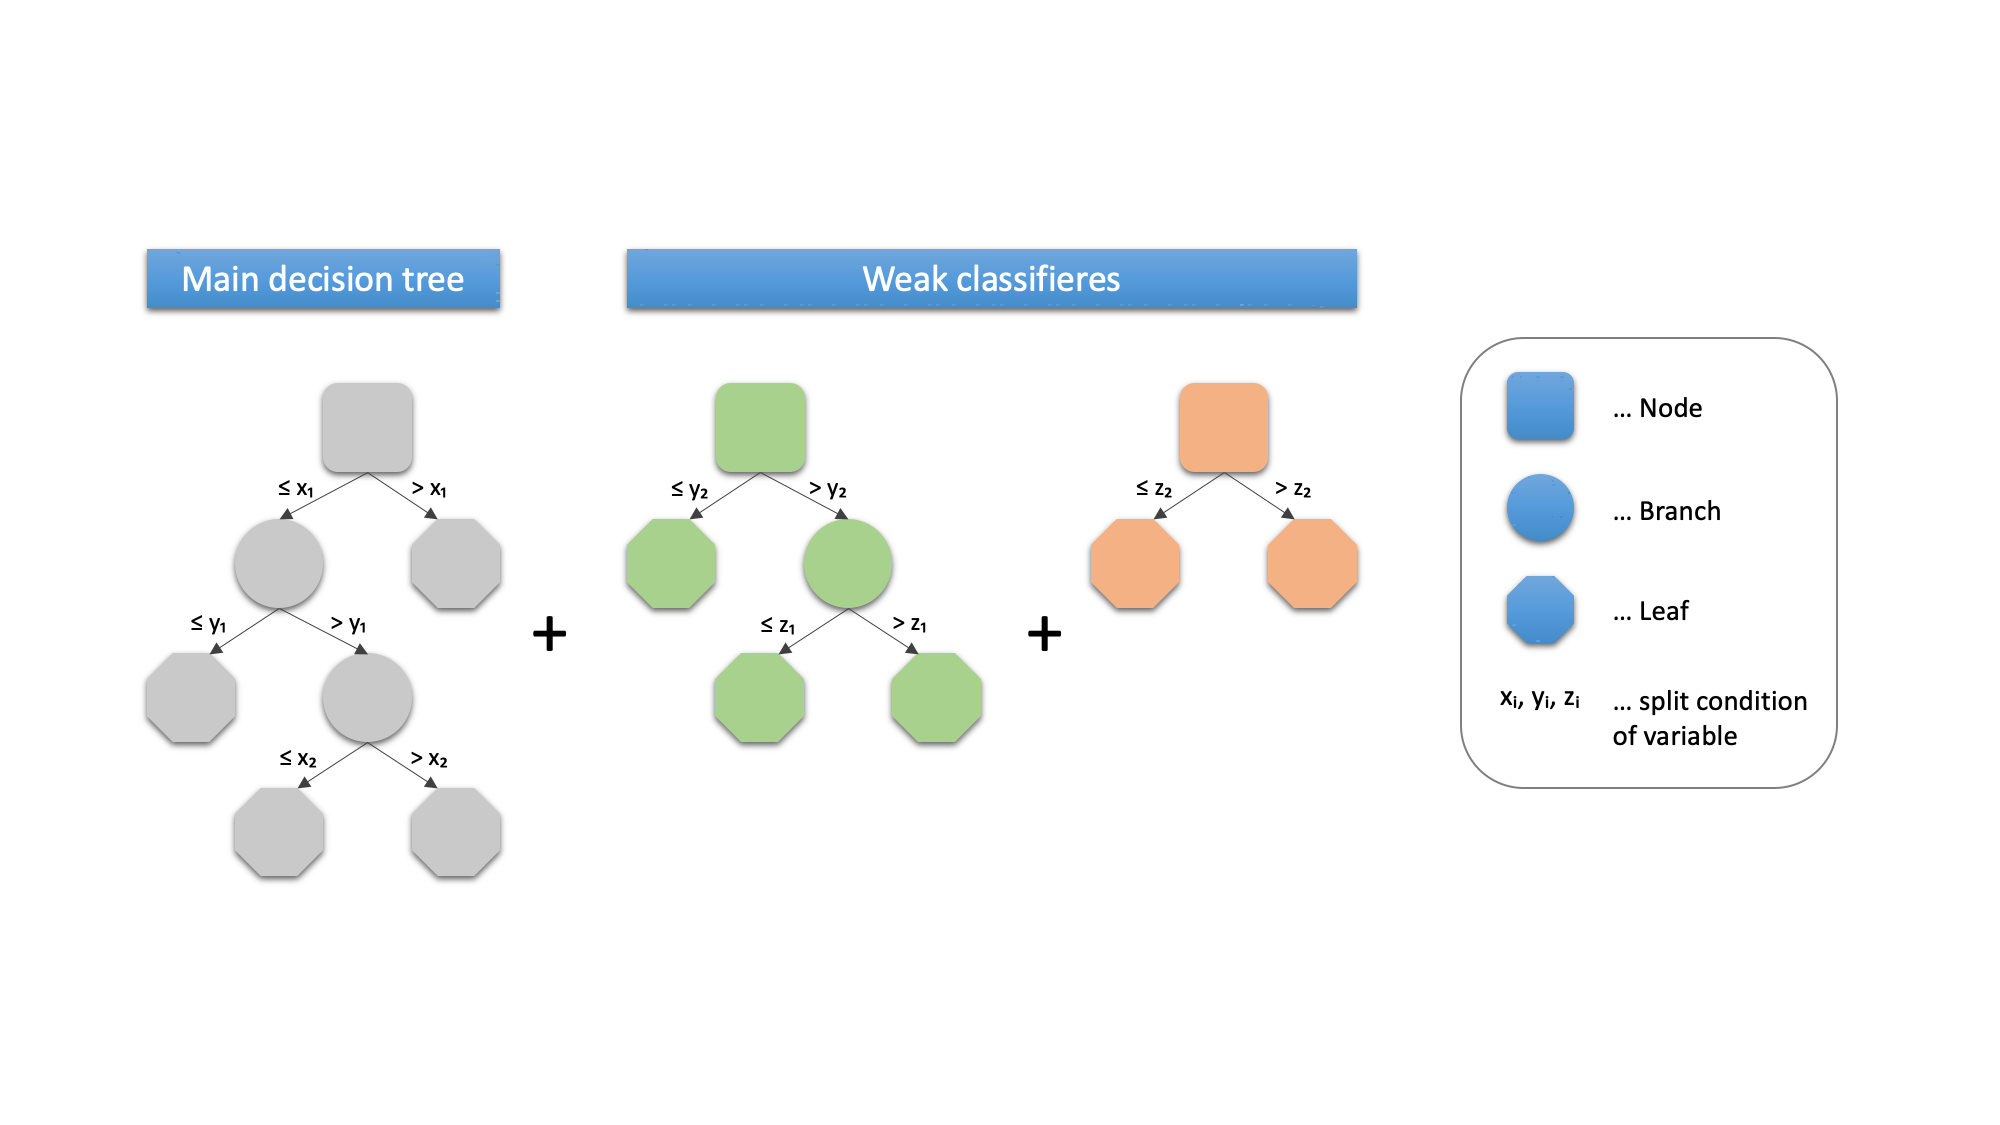
\includegraphics[width=1\textwidth]{figures/BDT.png}
	\caption{Outline of Boosted Decision Trees}
	\end{figure}
	
	\subsection{MLP - Multilayer Perceptron}
	
	The model is built out of multiple perceptrons, which are arranged in layers shown in Figure \ref{fig:MLP}. The value of one perceptron is the sum of all weighted inputs. This value is then transformed through an activation function and a treshhold. The activation funtion is a linear function for the input- and outputlayer, while it is usually the log-sigmoid transfer function for the hiddenlayers, as seen in Figure \ref{fig:log-sigmoid function}. All layers have a treshhold, except the inputlayer. 
	
	\begin{figure}[H]
	\centering
	\begin{minipage}{.5\textwidth}
	  \centering
	  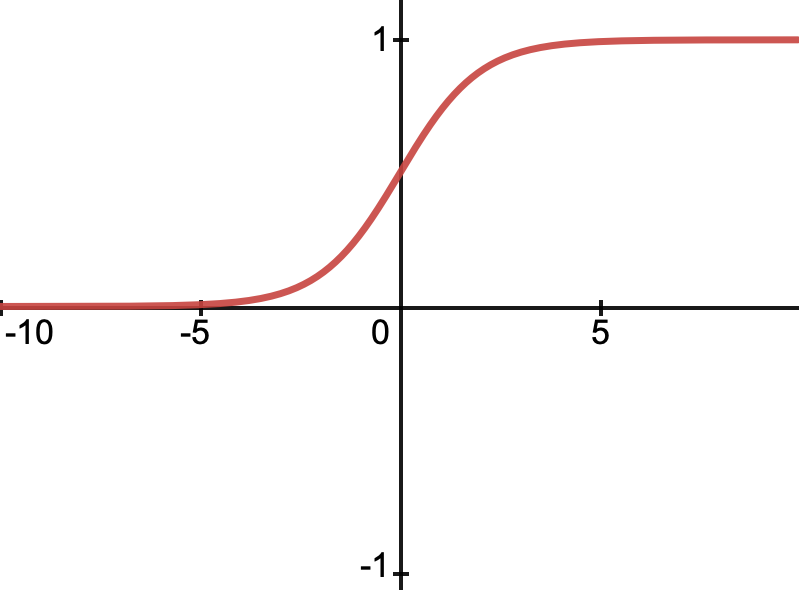
\includegraphics[width=0.5\linewidth]{figures/log-sigmoid.png}
	  %\captionof{figure}{log-sigmoid function}
	  %\label{fig:log-sigmoid function}
	\end{minipage}%
	\begin{minipage}{.5\textwidth}
	  \centering
		\begin{equation*}
			f(x) = \frac{1}{1 +e^{-x}}
		\end{equation*}
	  %\captionof{equation}{photonLepdR}
	\end{minipage}
	\captionof{figure}{log-sigmoid function}
	\label{fig:log-sigmoid function}
	\end{figure}
	
	In the MLP, every perceptron of a layer is connected to every perceptron of the previous and next layer. Each connection has an assigned weight, a so called weight coefficient. All coefficients of one layer can be written as a weight matrix. The first and last layer are called input- and outputlayer respectively, while the intermediate layers are the hiddenlayers. A MLP has a minimum of one hiddenlayer, therefore contains at least three layers~\cite{MLP08}.
	
	If the signal is only transmitted in one direction, therefore the MLP doesn't have any loops, it is described as feed forward. The learning process of the model is called backpropagation algorithm. It learns by minimizing the error between network output and expexted output. Initially, all weights are assigned random values, then every event will go through the network and the weights are adapted. Either all events will be put through the network first and then the values are adapted, or they are adjusted after each event, but for the latter the order of the events might be important. After one epoch the end criteria will be tested. If it fails, the whole learning process will be carried out again. If it is met, the algorithm is finished~\cite{MLP09}.
	
\begin{figure}[H]
	\begin{center}
	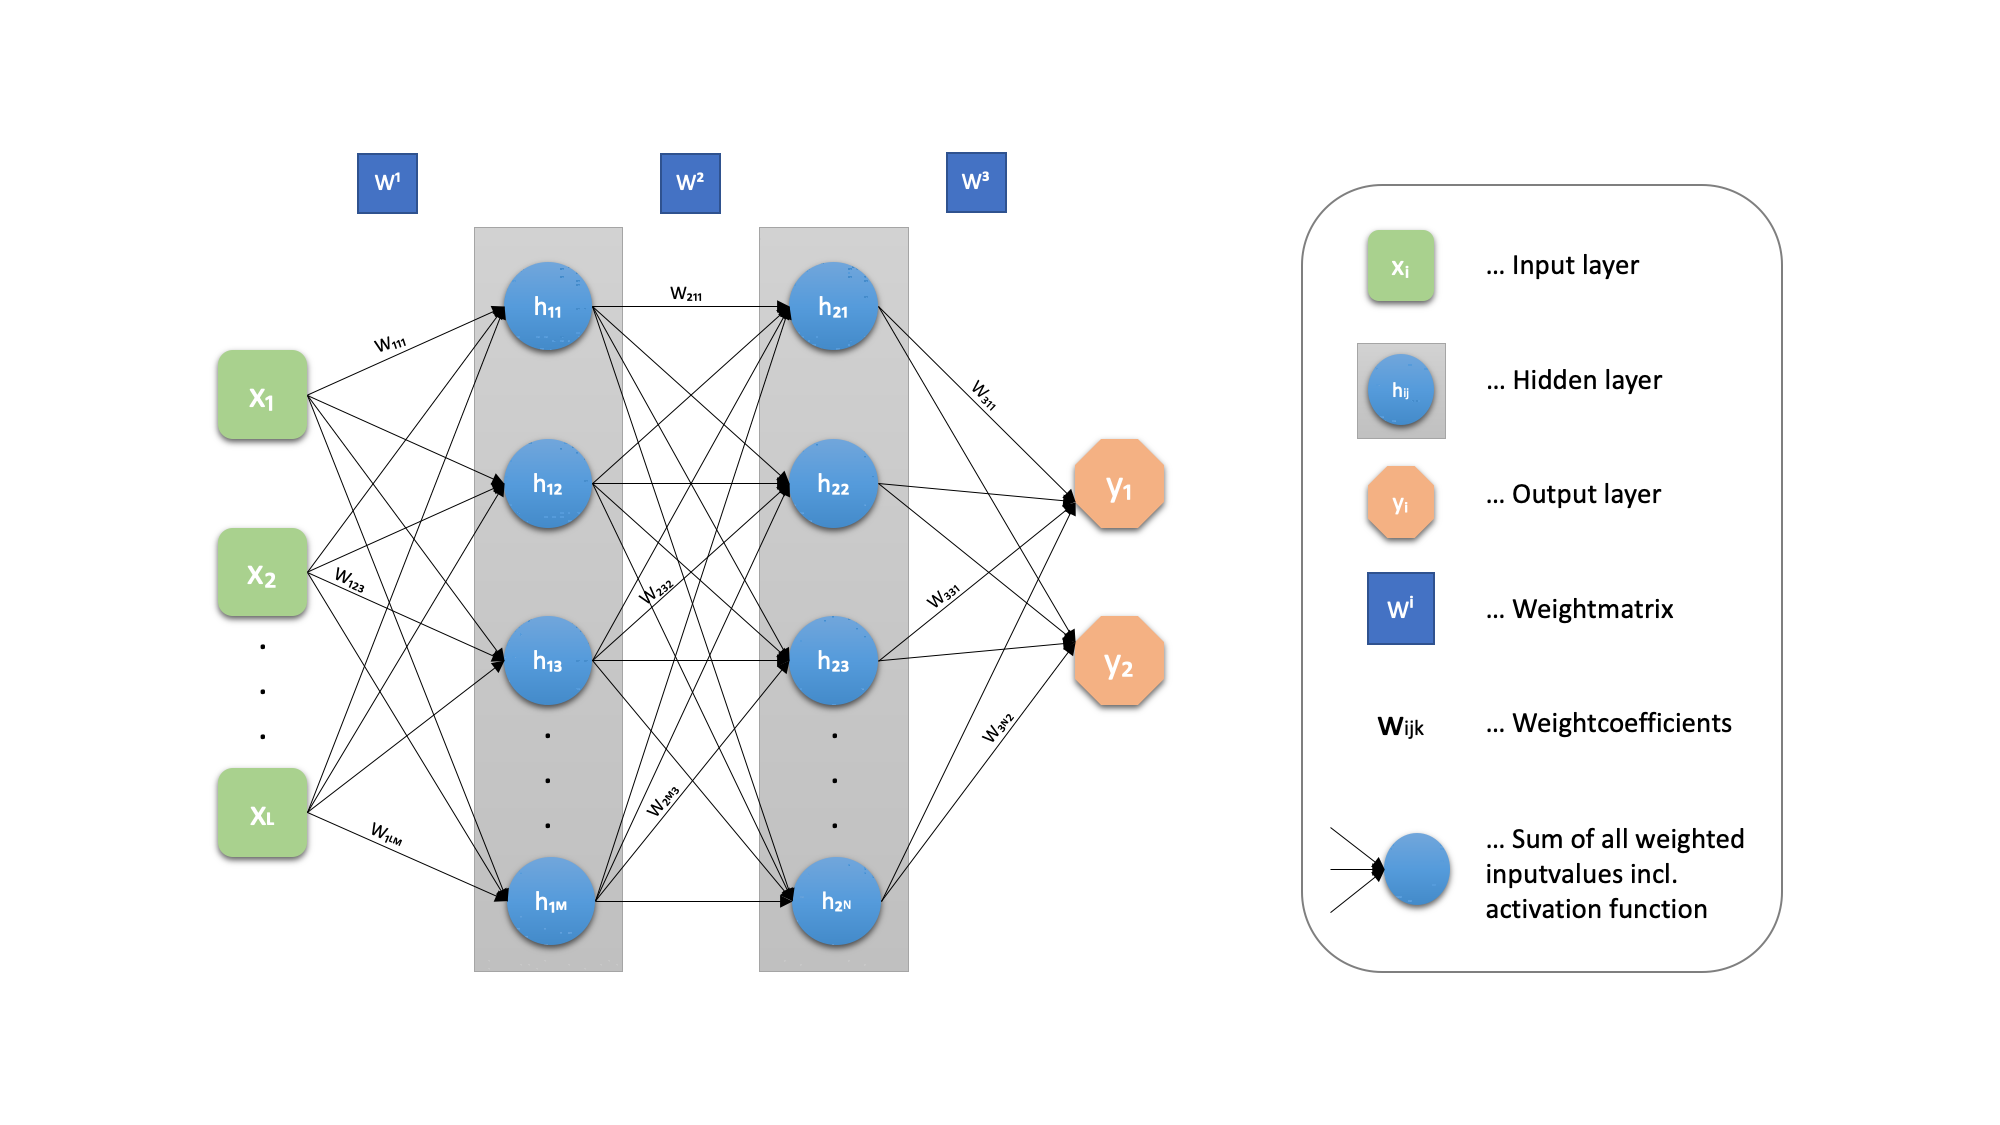
\includegraphics[width=1\textwidth]{figures/MLP.png}
	\caption{Outline of Multilayer Perceptron}
	\label{fig:MLP}
	\end{center}
\end{figure}

	\subsection{Training of MVA}
	
	The default values of the following configuration options were used for the models:
	
		\begin{itemize}
  			\item BDT
  					\begin{itemize}
  					\item Minimum percentage required in a leaf node (MinNodeSize): 5\%
  					\item Separation criterion for node splitting (SeparationType): GiniIndex
  					\end{itemize}
  		  	\item MLP
  					\begin{itemize}
  					\item Number of training cycles (NCycles): 500
  					\item ANN learning rate parameter (LearningRate): 0.02
  					\item Decay rate for learning parameter (DecayRate): 0.01
  					\item Neuron input function type (NeuronInputType): sum
  					\item Training Type (TrainingMethod): BP (Back-Propagation)
  					\end{itemize}		
		\end{itemize}
		
	A full list of all parameters, configuration options as well as their default values are given in the Annex, chapter \ref{sec:annex-BDTdef} and \ref{sec:annex-MLPdef}~\cite{TMVA}.
	
	These parameters were adapted to potentially improve the result:
		\begin{itemize}
  			\item BDT
  					\begin{itemize}
  					\item Maximum depth of decision trees allowed (MaxDepth)
  					\item Number of trees in the forest (NTrees)
  					\item Number of grid points used to find optimal cut (nCuts)
  					\end{itemize}
  		  	\item MLP
  					\begin{itemize}
  					\item Number of hidden layers (HiddenLayers)
  					\end{itemize}		
		\end{itemize}
		
	Their default values were used as a basis, listed in the second row in Table \ref{tab:config}. The MVAs were additionally trained with a lower and a higher configuration (row 2 and 3):
	
	\begin{table}[H]
	\begin{center}
	\begin{tabular}{|l|l|l|l|l|}
	\hline
	              & \multicolumn{3}{c|}{BDT}                         & \multicolumn{1}{c|}{MLP} \\ \hline
	Configuration & MaxDepth & NTrees & nCuts & HiddenLayers         \\ \hline
	1             & 1             & 400             & 10             & 5                        \\ \hline
	2             & 3             & 800             & 25             & 7                        \\ \hline
	3             & 5             & 1000            & 50             & 10                       \\ \hline
	\end{tabular}
		\caption{Configuration combinations used in MVAs}
		\label{tab:config}
	\end{center}
	\end{table}

	
The distribution and ROC-curves for the BDT- and MLP-models are shown for each selection and configuration in the following chapter. To avoid overfitting, each MVA is trained on one part of the sample (training sample) and tested on the rest (testing sample). If the results differ significantly, then this would be a sign of overfitting - the model only differentiates correctly on this specific sample. The results of the train- and test-sample can be seen in the distribution plots.

The ROC-curves (receiver operating characteristic curve) show the background rejection versus signal efficiency. The AUC (area under the ROC-curve) is used as a parameter to demonstrate how well a model performs. While discriminating between signal and background, the signal efficiency is the proportion of the correctly categorized signal events ($t\overline{t}\gamma$) and the background rejection is the correctly assigned fraction of background events ($t\overline{t}$). There are two types of errors during the distinction process:
		\begin{itemize}
  			\item a signal event is categorized as background, which is called false negative
  			\item a background event is assigned to the signal category, called false positive  			
  		\end{itemize}			
  		
Examples for different types of ROC-curves are displayed in Figure \ref{fig:ROC_ex}. The green curve indicate a good discriminatory power. The orange curve shows that the model assigns the events the wrong way around. If the ROC-curve follows the identity line, then the model doesn't have any discriminatory power.

	\begin{figure}[H]
	\centering
	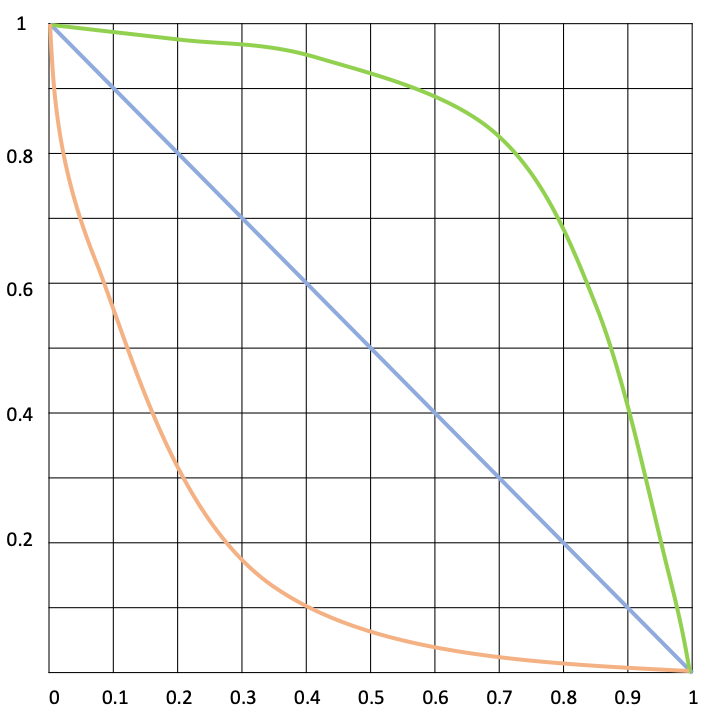
\includegraphics[width=0.5\textwidth]{figures/ROC_curve.png}
	\caption{ROC-curve examples}
	 \label{fig:ROC_ex}	
	\end{figure}
	
	\subsection{Results}
	
	The first set of selected variables (non-photon) were put into the models and are seen in Figure \ref{fig:ROC_s1_config1} - \ref{fig:ROC_s1_config3}. The ROC-curves indicate a slight improvement in the split between $t\overline{t}\gamma$- and $t\overline{t}$-events (blue line represents the identity line). At a signal efficiency of 70\%, a background rejection of about 40\% for MLP and 35\% for BDT can be achieved.
	
		In the second selection category, the currently used variable to differentiate between signal and background events was added (Figure \ref{fig:ROC_s2_config1} - \ref{fig:ROC_s2_config3}). The result has improved, the AUC increased significantly. At a signal efficiency of 70\%, a background rejection of about 46\% for MLP and 37\% for BDT can be achieved.
		
		Now adding the photon variables for the third selection shows a better success in the distinction process. They can be seen in Figure \ref{fig:ROC_s3_config1} - \ref{fig:ROC_s3_config3}. At a signal efficiency of 70\%, a background rejection of about 48\% for MLP and 38\% for BDT can be achieved.
		
		Between the three configuration combinations, there is only a slight difference for the MLP model, but for the BDT model there is an increase in the AUC for configuration 2 visible. Training- and testresults are nearly identical, so there are no signs of overfitting. The MLP model perfomed better than the BDT model for all selection categories. The third set of variables shows the best result.
				
	\begin{figure}[H]
	\centering
	\begin{minipage}{.5\textwidth}
	  \centering
	  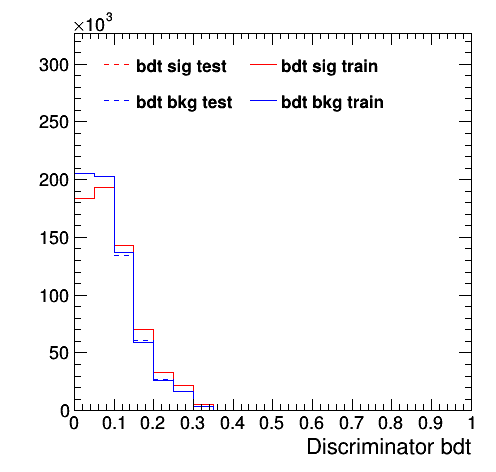
\includegraphics[width=0.75\linewidth]{figures/MVA/select1/config1/discriminator_bdt.png}
	  %\captionof{figure}{BDT distribution for selection 1 variables with configuration 1}
	  \label{fig:distr_s1_config1_bdt}
	\end{minipage}%
	\begin{minipage}{.5\textwidth}
	  \centering
	  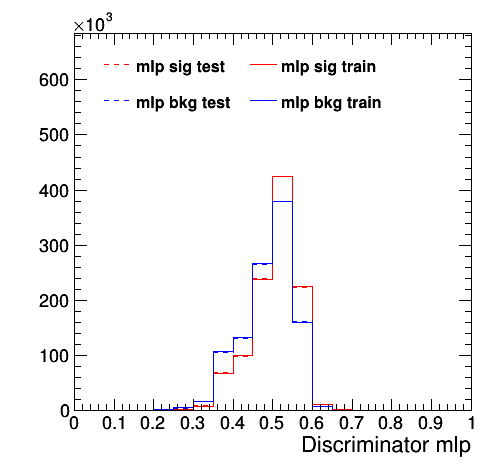
\includegraphics[width=0.75\linewidth]{figures/MVA/select1/config1/discriminator_mlp.png}
	  %\captionof{figure}{MLP distribution for selection 1 variables with configuration 1}
	  \label{fig:distr_s1_config1_mlp}
	\end{minipage}
	\centering
	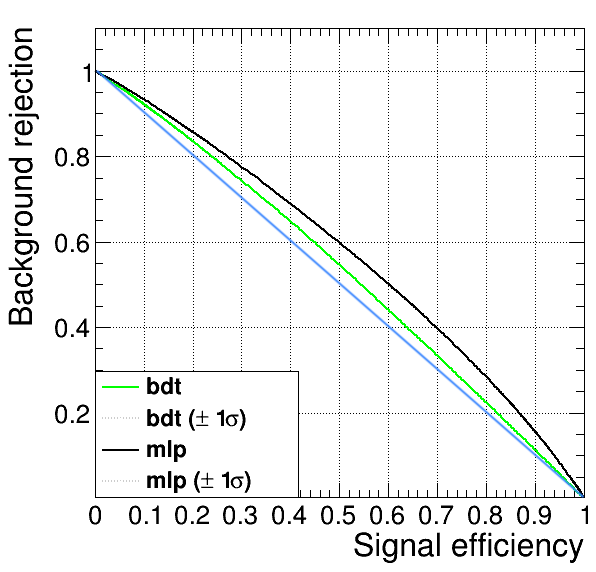
\includegraphics[width=0.5\textwidth]{figures/MVA/select1/config1/FOM_selection1_nL5_nT400_mD1_nC10.png}
	\caption{BDT-, MLP-distribution and ROC curve for variables from selection 1 with configuration 1}
	 \label{fig:ROC_s1_config1}
	\end{figure}
	
	\begin{figure}[H]
	\centering
	\begin{minipage}{.5\textwidth}
	  \centering
	  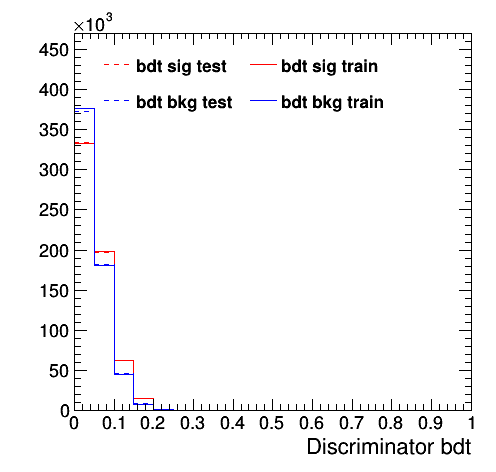
\includegraphics[width=0.75\linewidth]{figures/MVA/select1/config2/discriminator_bdt.png}
	  %\captionof{figure}{BDT distribution for selection 1 variables with configuration 2}
	  \label{fig:distr_s1_config2_bdt}
	\end{minipage}%
	\begin{minipage}{.5\textwidth}
	  \centering
	  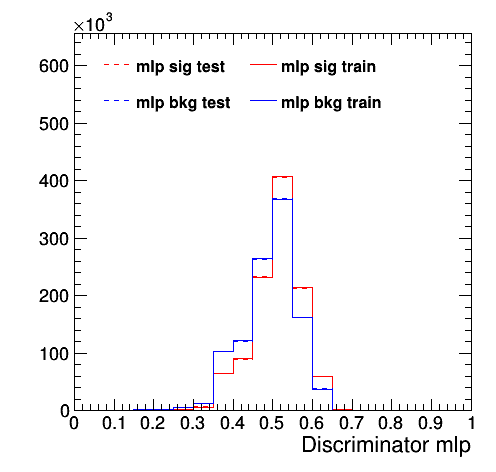
\includegraphics[width=0.75\linewidth]{figures/MVA/select1/config2/discriminator_mlp.png}
	  %\captionof{figure}{MLP distribution for selection 1 variables with configuration 2}
	  \label{fig:distr_s1_config2_mlp}
	\end{minipage}
	\centering
	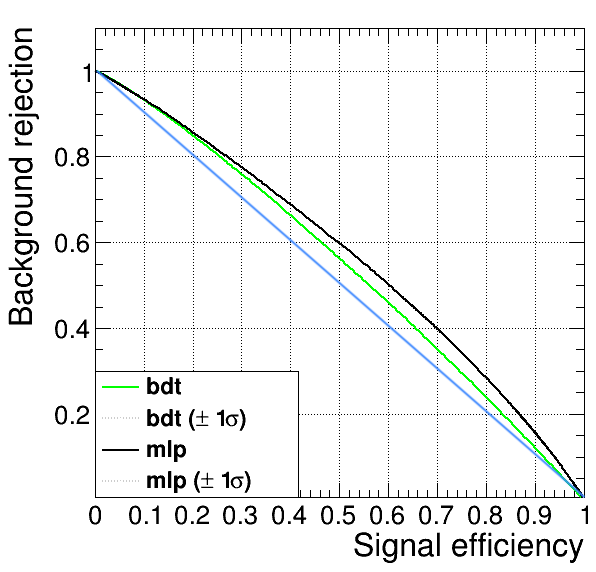
\includegraphics[width=0.5\textwidth]{figures/MVA/select1/config2/FOM_selection1_nL7_nT800_mD3_nC20.png}
	\caption{BDT-, MLP-distribution and ROC curve for variables from selection 1 with configuration 2}
	 \label{fig:ROC_s1_config2}
	\end{figure}
	
	\begin{figure}[H]
	\centering
	\begin{minipage}{.5\textwidth}
	  \centering
	  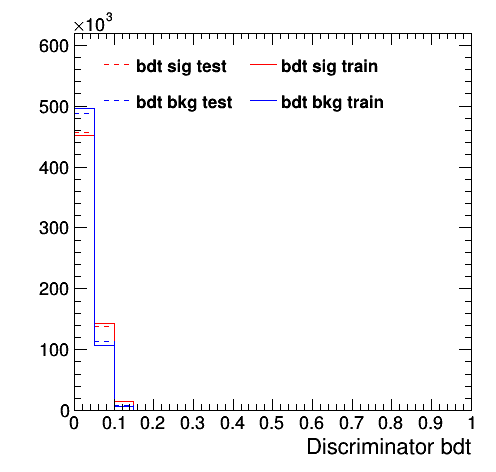
\includegraphics[width=0.75\linewidth]{figures/MVA/select1/config3/discriminator_bdt.png}
	  %\captionof{figure}{BDT distribution for selection 1 variables with configuration 3}
	  \label{fig:distr_s1_config3_bdt}
	\end{minipage}%
	\begin{minipage}{.5\textwidth}
	  \centering
	  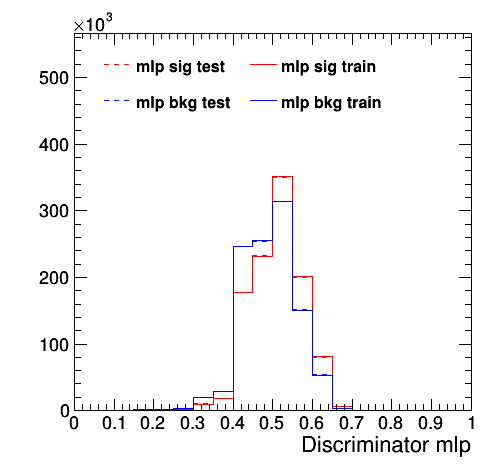
\includegraphics[width=0.75\linewidth]{figures/MVA/select1/config3/discriminator_mlp.png}
	  %captionof{figure}{MLP distribution for selection 1 variables with configuration 3}
	  \label{fig:distr_s1_config3_mlp}
	\end{minipage}
	\centering
	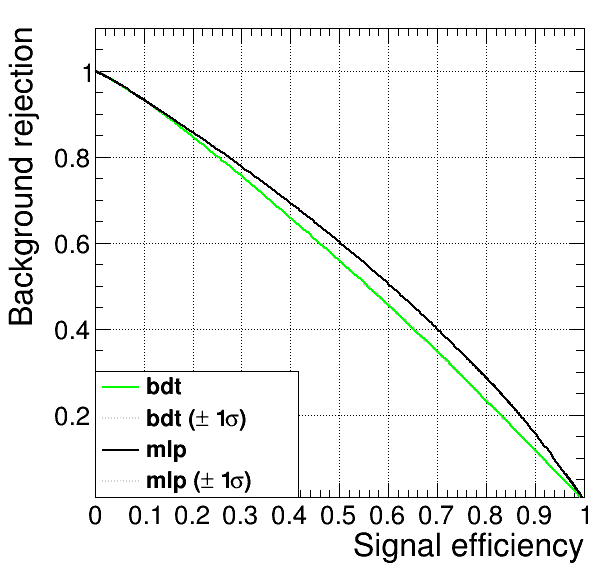
\includegraphics[width=0.5\textwidth]{figures/MVA/select1/config3/FOM_selection1_nL10_nT1000_mD5_nC50.png}
	\caption{BDT-, MLP-distribution and ROC curve for variables from selection 1 with configuration 3}
	 \label{fig:ROC_s1_config3}	
	\end{figure}

	
	\begin{figure}[H]
	\centering
	\begin{minipage}{.5\textwidth}
	  \centering
	  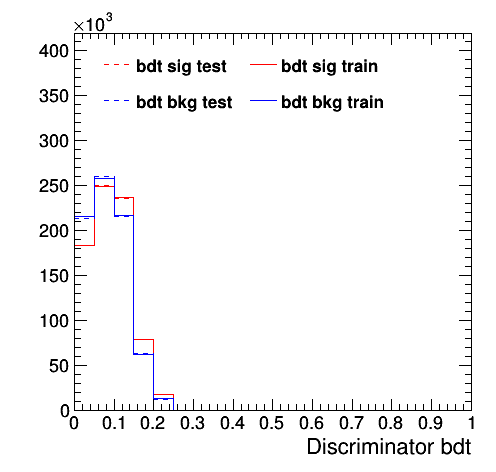
\includegraphics[width=0.75\linewidth]{figures/MVA/select2/config1/discriminator_bdt.png}
	  %\captionof{figure}{BDT distribution for selection 2 variables with configuration 1}
	  \label{fig:distr_s2_config1_bdt}
	\end{minipage}%
	\begin{minipage}{.5\textwidth}
	  \centering
	  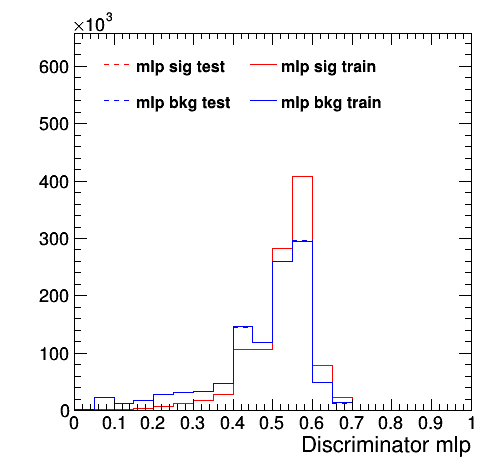
\includegraphics[width=0.75\linewidth]{figures/MVA/select2/config1/discriminator_mlp.png}
	  %\captionof{figure}{MLP distribution for selection 2 variables with configuration 1}
	  \label{fig:distr_s2_config1_mlp}
	\end{minipage}
	\centering
	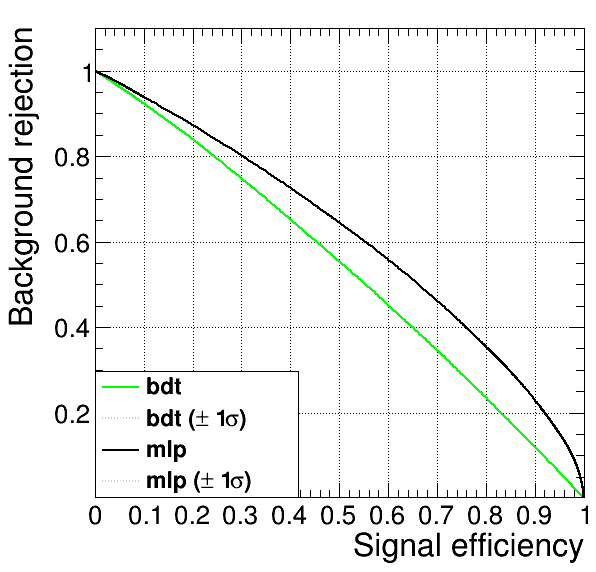
\includegraphics[width=0.5\textwidth]{figures/MVA/select2/config1/FOM_selection2_nL5_nT400_mD1_nC10.png}
	\caption{BDT-, MLP-distribution and ROC curve for variables from selection 2 with configuration 1}
	 \label{fig:ROC_s2_config1}
	\end{figure}
	
	\begin{figure}[H]
	\centering
	\begin{minipage}{.5\textwidth}
	  \centering
	  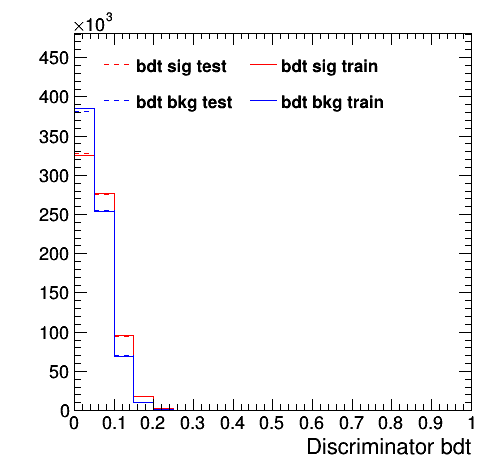
\includegraphics[width=0.75\linewidth]{figures/MVA/select2/config2/discriminator_bdt.png}
	  %\captionof{figure}{BDT distribution for selection 2 variables with configuration 2}
	  \label{fig:distr_s2_config2_bdt}
	\end{minipage}%
	\begin{minipage}{.5\textwidth}
	  \centering
	  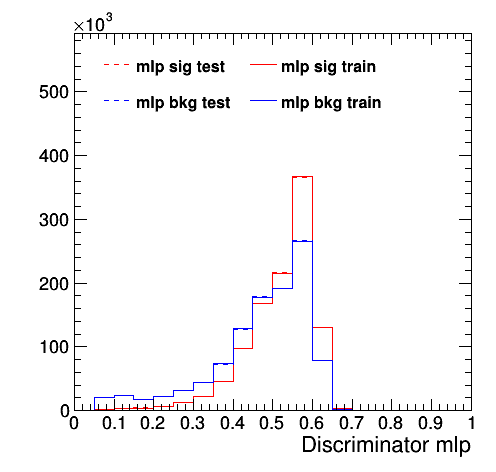
\includegraphics[width=0.75\linewidth]{figures/MVA/select2/config2/discriminator_mlp.png}
	  %\captionof{figure}{MLP distribution for selection 2 variables with configuration 2}
	  \label{fig:distr_s2_config2_mlp}
	\end{minipage}
	\centering
	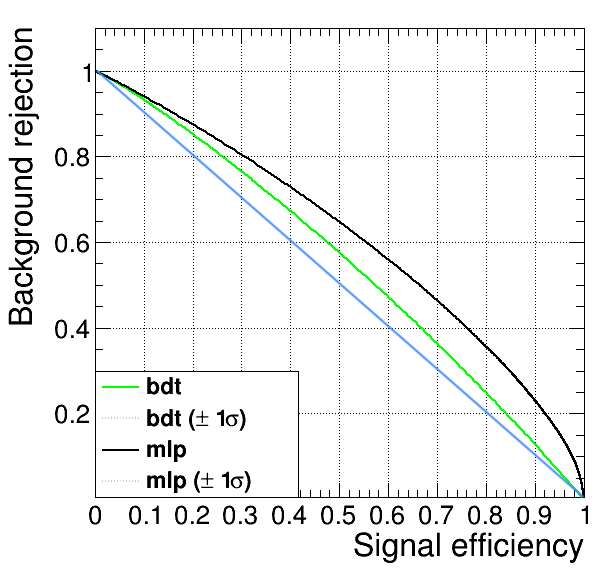
\includegraphics[width=0.5\textwidth]{figures/MVA/select2/config2/FOM_selection2_nL7_nT800_mD3_nC20.png}
	\caption{BDT-, MLP-distribution and ROC curve for variables from selection 2 with configuration 2}
	 \label{fig:ROC_s2_config2}	
	\end{figure}
	
	\begin{figure}[H]
	\centering
	\begin{minipage}{.5\textwidth}
	  \centering
	  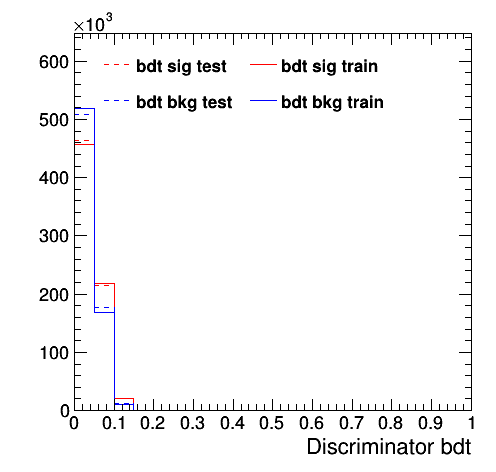
\includegraphics[width=0.75\linewidth]{figures/MVA/select2/config3/discriminator_bdt.png}
	  %\captionof{figure}{BDT distribution for selection 2 variables with configuration 3}
	  \label{fig:distr_s2_config3_bdt}
	\end{minipage}%
	\begin{minipage}{.5\textwidth}
	  \centering
	  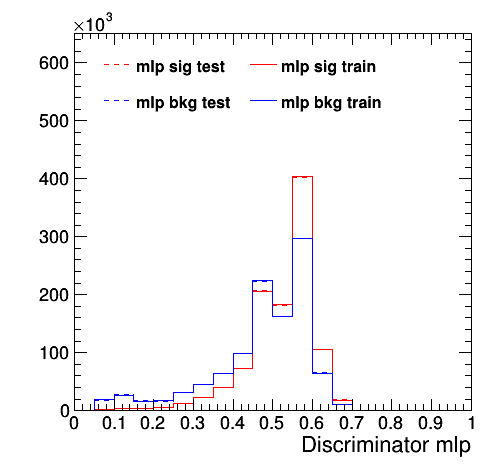
\includegraphics[width=0.75\linewidth]{figures/MVA/select2/config3/discriminator_mlp.png}
	  %\captionof{figure}{MLP distribution for selection 2 variables with configuration 3}
	  \label{fig:distr_s2_config3_mlp}
	\end{minipage}
	\centering
	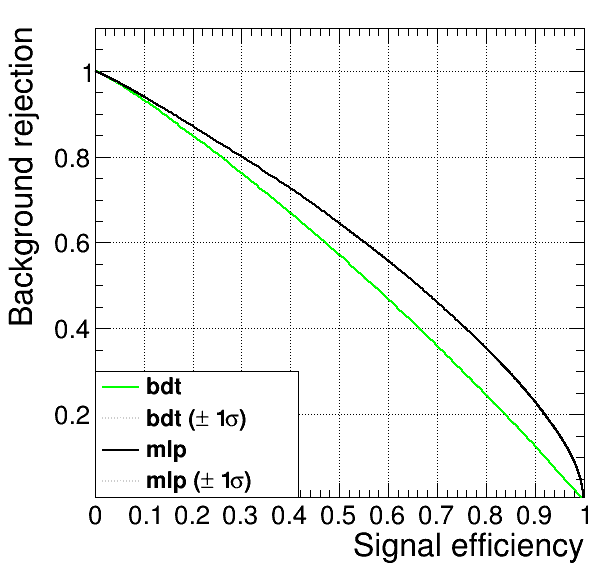
\includegraphics[width=0.5\textwidth]{figures/MVA/select2/config3/FOM_selection2_nL10_nT1000_mD5_nC50.png}
	\caption{BDT-, MLP-distribution and ROC curve for variables from selection 2 with configuration 3}
	 \label{fig:ROC_s2_config3}	
	\end{figure}
	
	
	\begin{figure}[H]
	\centering
	\begin{minipage}{.5\textwidth}
	  \centering
	  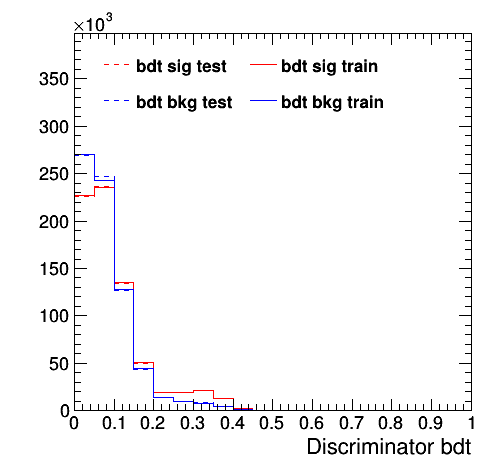
\includegraphics[width=0.75\linewidth]{figures/MVA/select3/config1/discriminator_bdt.png}
	  %\captionof{figure}{BDT distribution for selection 3 variables with configuration 1}
	  \label{fig:distr_s3_config1_bdt}
	\end{minipage}%
	\begin{minipage}{.5\textwidth}
	  \centering
	  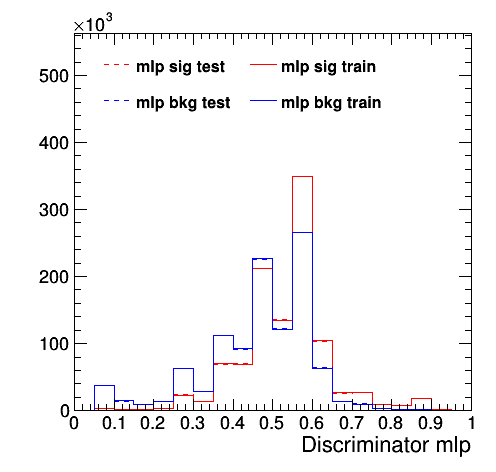
\includegraphics[width=0.75\linewidth]{figures/MVA/select3/config1/discriminator_mlp.png}
	  %\captionof{figure}{MLP distribution for selection 3 variables with configuration 1}
	  \label{fig:distr_s3_config1_mlp}
	\end{minipage}
	\centering
	\includegraphics[width=0.5\textwidth]{figures/MVA/select3/config1/FOM_selection3_nL5_nT400_mD1_nC10.png}
	\caption{BDT-, MLP-distribution and ROC curve for variables from selection 3 with configuration 1}
	 \label{fig:ROC_s3_config1}
	\end{figure}
	
	\begin{figure}[H]
	\centering
	\begin{minipage}{.5\textwidth}
	  \centering
	  \includegraphics[width=0.75\linewidth]{figures/MVA/select3/config2/discriminator_bdt.png}
	  %\captionof{figure}{BDT distribution for selection 3 variables with configuration 2}
	  \label{fig:distr_s3_config2_bdt}
	\end{minipage}%
	\begin{minipage}{.5\textwidth}
	  \centering
	  \includegraphics[width=0.75\linewidth]{figures/MVA/select3/config2/discriminator_mlp.png}
	  %\captionof{figure}{MLP distribution for selection 3 variables with configuration 2}
	  \label{fig:distr_s3_config2_mlp}
	\end{minipage}
	\centering
	\includegraphics[width=0.5\textwidth]{figures/MVA/select3/config2/FOM_selection3_nL7_nT800_mD3_nC20.png}
	\caption{BDT-, MLP-distribution and ROC curve for variables from selection 3 with configuration 2}
	 \label{fig:ROC_s3_config2}	
	\end{figure}
	
	\begin{figure}[H]
	\centering
	\begin{minipage}{.5\textwidth}
	  \centering
	  \includegraphics[width=0.75\linewidth]{figures/MVA/select3/config3/discriminator_bdt.png}
	  %\captionof{figure}{BDT distribution for selection 3 variables with configuration 3}
	  \label{fig:distr_s3_config3_bdt}
	\end{minipage}%
	\begin{minipage}{.5\textwidth}
	  \centering
	  \includegraphics[width=0.75\linewidth]{figures/MVA/select3/config3/discriminator_mlp.png}
	  %\captionof{figure}{MLP distribution for selection 3 variables with configuration 3}
	  \label{fig:distr_s3_config3_mlp}
	\end{minipage}
	\centering
	\includegraphics[width=0.5\textwidth]{figures/MVA/select3/config3/FOM_selection3_nL10_nT1000_mD5_nC50.png}
	\caption{BDT-, MLP-distribution and ROC curve for variables from selection 3 with configuration 3}
	 \label{fig:ROC_s3_config3}	
	\end{figure}
				
\section{Conclusion}
It is very difficult to differentiate between $t\overline{t}\gamma$ and $t\overline{t}$ events because they show very similiar behaviour in the signal region. Nevertheless, a slight improvement was possible by training a MVA with relevant variables. At a signal efficiency of 70\%, a background rejection of up to 48\% for MLP and up to 38\% for BDT can be achieved. Especially photon variables provide a bigger improvement. MLPs show a better performance than BDTs with a 5-10\% difference observed in background rejection at 70\% signal efficiency, which suggests the selection of this type of model.

\appendix
\section{Appendix}
	\subsection{Full list of variables with almost identical distributions}
	\label{sec:annex-identical}
	\begin{figure}[H]
	\centering
	\begin{minipage}{.5\textwidth}
	  \centering
	  \includegraphics[width=0.7\linewidth]{figures/Notused/Bj0_eta.png}
	  %\captionof{figure}{Bj0\_eta}
	\end{minipage}%
	\begin{minipage}{.5\textwidth}
	  \centering
	  \includegraphics[width=0.7\linewidth]{figures/Notused/Bj0_phi.png}
	  %\captionof{figure}{Bj0\_phi}
	\end{minipage}
	  \captionof{figure}{pseudorapidity and $\Delta\phi$ of first b-jet suggest no discriminatory power}	
	\end{figure}
	
	\begin{figure}[H]
	\centering
	\begin{minipage}{.5\textwidth}
	  \centering
	  \includegraphics[width=0.7\linewidth]{figures/Notused/Bj0_pt.png}
	  %\captionof{figure}{Bj0\_pt}
	\end{minipage}%
	\begin{minipage}{.5\textwidth}
	  \centering
	  \includegraphics[width=0.7\linewidth]{figures/Notused/Bj1_eta.png}
	  %\captionof{figure}{Bj1\_eta}
	\end{minipage}
	  \captionof{figure}{transverse momentum of first b-jet and pseudorapidity of second b-jet suggest no discriminatory power}	
	\end{figure}
	
	\begin{figure}[H]
	\centering
	\begin{minipage}{.5\textwidth}
	  \centering
	  \includegraphics[width=0.7\linewidth]{figures/Notused/Bj1_phi.png}
	  %\captionof{figure}{Bj1\_phi}
	\end{minipage}%
	\begin{minipage}{.5\textwidth}
	  \centering
	  \includegraphics[width=0.7\linewidth]{figures/Notused/Bj1_pt.png}
	  %\captionof{figure}{Bj1\_pt}
	\end{minipage}
	  \captionof{figure}{$\Delta\phi$ and transverse momentum of second b-jet suggest no discriminatory power}	
	\end{figure}
	
	\begin{figure}[H]
	\centering
	\begin{minipage}{.5\textwidth}
	  \centering
	  \includegraphics[width=0.7\linewidth]{figures/Notused/JetGood0_btagDeepB.png}
	  %\captionof{figure}{JetGood0\_btagDeepB}
	\end{minipage}%
	\begin{minipage}{.5\textwidth}
	  \centering
	  \includegraphics[width=0.7\linewidth]{figures/Notused/JetGood1_btagDeepB.png}
	  %\captionof{figure}{JetGood1\_btagDeepB}
	\end{minipage}
	  \captionof{figure}{results of neural network to identify first and second b-jet suggest no discriminatory power}	
	\end{figure}
	
	\begin{figure}[H]
	\centering
	\begin{minipage}{.5\textwidth}
	  \centering
	  \includegraphics[width=0.7\linewidth]{figures/Notused/JetGood0_chHEF.png}
	  %\captionof{figure}{JetGood0\_chHEF}
	\end{minipage}%
	\begin{minipage}{.5\textwidth}
	  \centering
	  \includegraphics[width=0.7\linewidth]{figures/Notused/JetGood0_chEmEF.png}
	  %\captionof{figure}{JetGood0\_chEmEF}
	\end{minipage}
	  \captionof{figure}{proportion of energy coming from charged particles detected in HCAL and detected in ECAL suggest no discriminatory power}			
	\end{figure}
	
	\begin{figure}[H]
	\centering
	\begin{minipage}{.5\textwidth}
	  \centering
	  \includegraphics[width=0.7\linewidth]{figures/Notused/JetGood0_neHEF.png}
	  %\captionof{figure}{JetGood0\_neHEF}
	\end{minipage}%
	\begin{minipage}{.5\textwidth}
	  \centering
	  \includegraphics[width=0.7\linewidth]{figures/Notused/JetGood0_neEmEF.png}
	  %\captionof{figure}{JetGood0\_neEmEF}
	\end{minipage}
	  \captionof{figure}{proportion of energy coming from neutral particles detected in HCAL and detected in ECAL suggest no discriminatory power}			
	\end{figure}
	
	\begin{figure}[H]
	\centering
	\begin{minipage}{.5\textwidth}
	  \centering
	  \includegraphics[width=0.7\linewidth]{figures/Notused/JetGood1_eta.png}
	  %\captionof{figure}{JetGood1\_eta}
	\end{minipage}%
	\begin{minipage}{.5\textwidth}
	  \centering
	  \includegraphics[width=0.7\linewidth]{figures/Notused/JetGood1_phi.png}
	  %\captionof{figure}{JetGood1\_phi}
	\end{minipage}
	  \captionof{figure}{pseudorapidity and $\Delta\phi$ of second jet suggest no discriminatory power}	
	\end{figure}
	
	\begin{figure}[H]
	\centering
	\begin{minipage}{.5\textwidth}
	  \centering
	  \includegraphics[width=0.7\linewidth]{figures/Notused/JetGood1_pt.png}
	  %\captionof{figure}{JetGood1\_pt}
	\end{minipage}%
	\begin{minipage}{.5\textwidth}
	  \centering
	  \includegraphics[width=0.7\linewidth]{figures/Notused/LeptonTight0__phi.png}
	  %\captionof{figure}{LeptonTight0\_phi}
	\end{minipage}
	  \captionof{figure}{transverse momentum of second jet and $\Delta\phi$ of lepton suggest no discriminatory power}	
	\end{figure}
	
	\begin{figure}[H]
	\centering
	\begin{minipage}{.5\textwidth}
	  \centering
	  \includegraphics[width=0.7\linewidth]{figures/Notused/LeptonTight0_eta.png}
	  %\captionof{figure}{LeptonTight0\_eta}
	\end{minipage}%
	\begin{minipage}{.5\textwidth}
	  \centering
	  \includegraphics[width=0.7\linewidth]{figures/Notused/LeptonTight0_pfRelIso03_all.png}
	  %\captionof{figure}{LeptonTight0\_pfRelIso03\_all}
	\end{minipage}
	  \captionof{figure}{pseudorapidity of lepton and relative isolation of lepton to all particles suggest no discriminatory power}	
	\end{figure}
	
	\begin{figure}[H]
	\centering
	\begin{minipage}{.5\textwidth}
	  \centering
	  \includegraphics[width=0.7\linewidth]{figures/Notused/LeptonTight0_pfRelIso03_chg.png}
	  %\captionof{figure}{LeptonTight0\_pfRelIso03\_chg}
	\end{minipage}%
	\begin{minipage}{.5\textwidth}
	  \centering
	  \includegraphics[width=0.7\linewidth]{figures/Notused/LeptonTight0_pfRelIso03_ne.png}
	  %\captionof{figure}{LeptonTight0\_pfRelIso03\_ne}
	\end{minipage}
	  \captionof{figure}{relative isolation of lepton to charged and neutral particles suggest no discriminatory power}	
	\end{figure}
	
	\begin{figure}[H]
	\centering
	\begin{minipage}{.5\textwidth}
	  \centering
	  \includegraphics[width=0.7\linewidth]{figures/Notused/LeptonTight0_pt.png}
	  %\captionof{figure}{LeptonTight0\_pt}
	\end{minipage}%
	\begin{minipage}{.5\textwidth}
	  \centering
	  \includegraphics[width=0.7\linewidth]{figures/Notused/nElectronTight.png}
	  %\captionof{figure}{nElectronTight}
	\end{minipage}
	  \captionof{figure}{transverse momentum of lepton and number of electrons suggest no discriminatory power}	
	\end{figure}
	
	\begin{figure}[H]
	\centering
	\begin{minipage}{.5\textwidth}
	  \centering
	  \includegraphics[width=0.7\linewidth]{figures/Notused/nHighPTPhotons.png}
	  %\captionof{figure}{nHighPTPhotons}
	\end{minipage}%
	\begin{minipage}{.5\textwidth}
	  \centering
	  \includegraphics[width=0.7\linewidth]{figures/Notused/nJet.png}
	  %\captionof{figure}{nJet}
	\end{minipage}
	  \captionof{figure}{number of photons with high p\textsubscript{T} and number of jets suggest no discriminatory power}	
	\end{figure}
	
	\begin{figure}[H]
	\centering
	\begin{minipage}{.5\textwidth}
	  \centering
	  \includegraphics[width=0.7\linewidth]{figures/Notused/nLeptonTight.png}
	  %\captionof{figure}{nLeptonTight}
	\end{minipage}%
	\begin{minipage}{.5\textwidth}
	  \centering
	  \includegraphics[width=0.7\linewidth]{figures/Notused/nMuonTight.png}
	  %\captionof{figure}{nMuonTight}
	\end{minipage}
	  \captionof{figure}{number of leptons and muons suggest no discriminatory power}	
	\end{figure}
	
	\begin{figure}[H]
		\begin{center}
		\includegraphics[width=0.35\textwidth]{figures/Notused/nPhotonGood.png}
		\caption{number of photons suggests no discriminatory power}	
		\end{center}
	\end{figure}
	
	\subsection{Configuration options for MVA method: BDT}
	
	Note: Table taken from~\cite{TMVA}, p. 116-118.
	
	\label{sec:annex-BDTdef}
	
\begin{longtable}[c]{|p{4cm}|p{2.5cm}|p{7cm}|}
\hline
Option               & Default                & Description                                                                                                                                                                                                                                                                                             \\ \hline
NTrees               & 800                    & Number of trees in the forest                                                                                                                                                                                                                                                                           \\ \hline
MaxDepth             & 3                      & Max depth of the decision tree allowed                                                                                                                                                                                                                                                                  \\ \hline
MinNodeSize          & 5\%                    & Minimum percentage of training events required in a leaf node (default: Classification: 5\%, Regression: 0.2\%)                                                                                                                                                                                         \\ \hline
nCuts                & 20                     & Number of grid points in variable range used in finding optimal cut in node splitting                                                                                                                                                                                                                   \\ \hline
BoostType            & AdaBoost               & Boosting type for the trees in the forest (note: AdaCost is still experimental) (AdaBoost, RealAdaBoost, Bagging, AdaBoostR2, Grad)                                                                                                                                                                     \\ \hline
AdaBoostR2Loss       & Quadratic              & Type of Loss function in AdaBoostR2 (Linear, Quadratic, Exponential)                                                                                                                                                                                                                                    \\ \hline
UseBaggedGrad        & False                  & Use only a random subsample of all events for growing the trees in each iteration. (Only valid for GradBoost)                                                                                                                                                                                           \\ \hline
Shrinkage            & 1                      & Learning rate for GradBoost algorithm                                                                                                                                                                                                                                                                   \\ \hline
AdaBoostBeta         & 0.5                    & Learning rate for AdaBoost algorithm                                                                                                                                                                                                                                                                    \\ \hline
UseRandomisedTrees   & False                  & Determine at each node splitting the cut variable only as the best out of a random subset of variables (like in RandomForests)                                                                                                                                                                          \\ \hline
UseNvars             & 2                      & Size of the subset of variables used with RandomisedTree option                                                                                                                                                                                                                                         \\ \hline
UsePoissonNvars      & True                   & Interpret UseNvars not as fixed number but as mean of a Possion distribution in each split with RandomisedTree option                                                                                                                                                                                   \\ \hline
BaggedSampleFraction & 0.6                    & Relative size of bagged event sample to original size of the data sample (used whenever bagging is used (i.e. Use-BaggedGrad, Bagging, ..))                                                                                                                                                             \\ \hline
UseYesNoLeaf         & True                   & Use Sig or Bkg categories, or the purity=S/(S+B) as classification of the leaf node -\textgreater Real-AdaBoost                                                                                                                                                                                         \\ \hline
NegWeightTreatment   & InverseBoost-NegWeights & How to treat events with negative weights in the BDT training (particular the boosting) : IgnoreInTraining; Boost With inverse boostweight (InverseBoostNegWeights); Pair events with negative and positive weights in traning sample and *annihilate* them (PairNegWeightsGlobal, experimental!), Pray \\ \hline
NodePurityLimit      & 0.5                    & In boosting/pruning, nodes with purity \textgreater NodePurityLimit are signal; background otherwise.                                                                                                                                                                                                   \\ \hline
SeparationType       & GiniIndex              & Separation criterion for node splitting (CrossEntropy, GiniIndex, GiniIndexWithLaplace, MisClassificationError, SdivSqrtSPlusB, RegressionVariance)                                                                                                                                                     \\ \hline
DoBoostMonitor       & False                  & Create control plot with ROC integral vs tree number                                                                                                                                                                                                                                                    \\ \hline
UseFisherCuts        & False                  & Use multivariate splits using the Fisher criterion                                                                                                                                                                                                                                                      \\ \hline
MinLinCorrForFisher  & 0.8                    & The minimum linear correlation between two variables demanded for use in Fisher criterion in node splitting                                                                                                                                                                                             \\ \hline
UseExclusiveVars     & False                  & Variables already used in fisher criterion are not anymore analysed individually for node splitting                                                                                                                                                                                                     \\ \hline
DoPreselection       & False                  & Apply automatic pre-selection for 100\% efficient signal (bkg) cuts prior to training                                                                                                                                                                                                                   \\ \hline
RenormByClass        & False                  & Individually re-normalize each event class to the original size after boosting                                                                                                                                                                                                                          \\ \hline
SigToBkgFraction     & 1                      & Sig to Bkg ratio used in Training (similar to NodePurityLimit, which cannot be used in real adaboost)                                                                                                                                                                                                   \\ \hline
PruneMethod          & NoPruning              & Note: for BDTs use small trees (e.g.MaxDepth=3) and NoPruning; Pruning: Method used for pruning (removal) of statistically insignificant branches (NoPruning, ExpectedError, CostComplexity)                                                                                                            \\ \hline
PruneStrength        & 0                      & Pruning strength                                                                                                                                                                                                                                                                                        \\ \hline
PruningValFraction   & 0.5                    & Fraction of events to use for optimizing automatic pruning.                                                                                                                                                                                                                                             \\ \hline
nEventsMin           & 0                      & deprecated: Use MinNodeSize (in \% of training events) instead                                                                                                                                                                                                                                          \\ \hline
GradBaggingFraction  & 0.6                    & deprecated: Use *BaggedSampleFraction* instead: Defines the fraction of events to be used in each iteration, e.g. when UseBaggedGrad=kTRUE.                                                                                                                                                             \\ \hline
UseNTrainEvents      & 0                      & deprecated: Use *BaggedSampleFraction* instead: Number of randomly picked training events used in randomised (and bagged) trees                                                                                                                                                                         \\ \hline
NNodesMax            & 0                      & deprecated: Use MaxDepth instead to limit the tree size                                                                                                                                                                                                                                                 \\ \hline

	\caption{Full list of configuration options and their default values (BDT)}
\end{longtable}

	\subsection{Configuration options for MVA method: MLP}
	Note: Table taken from~\cite{TMVA}, p. 98-99.
	
	\label{sec:annex-MLPdef}
	
\begin{longtable}[c]{|p{4cm}|p{2.5cm}|p{7cm}|}

\hline
Option             & Default    & Description                                                                                                                                            \\ \hline
NCycles            & 500        & Number of training cycles                                                                                                                              \\ \hline
HiddenLayers       & N,N-1      & Specification of hidden layer architecture                                                                                                             \\ \hline
NeuronType         & sigmoid    & Neuron activation function type                                                                                                                        \\ \hline
RandomSeed         & 1          & Random seed for initial synapse weights (0 means unique seed for each run; default value ’1’)                                                          \\ \hline
EstimatorType      & MSE        & MSE (Mean Square Estimator) for Gaussian Likelihood or CE (Cross- Entropy) for Bernoulli Likelihood, linear, sigmoid, tanh, radial                     \\ \hline
NeuronInputType    & sum        & Neuron input function type (sum, sqsum, abssum)                                                                                                        \\ \hline
TrainingMethod     & BP         & Train with Back-Propagation (BP), BFGS Algorithm (BFGS), or Genetic Algorithm (GA - slower and worse)                                                  \\ \hline
LearningRate       & 0.02       & ANN learning rate parameter                                                                                                                            \\ \hline
DecayRate          & 0.01       & Decay rate for learning parameter                                                                                                                      \\ \hline
TestRate           & 10         & Test for overtraining performed at each \#th epochs                                                                                                    \\ \hline
EpochMonitoring    & False      & Provide epoch-wise monitoring plots according to TestRate (caution: causes big ROOT output file!)                                                      \\ \hline
Sampling           & 1          & Only ’Sampling’ (randomly selected) events are trained each epoch                                                                                      \\ \hline
SamplingEpoch      & 1          & Sampling is used for the first ’SamplingEpoch’ epochs, afterwards, all events are taken for training                                                   \\ \hline
SamplingImportance & 1          & The sampling weights of events in epochs which successful (worse estimator than before) are multiplied with SamplingImportance, else they are divided. \\ \hline
SamplingTraining   & True       & The training sample is sampled                                                                                                                         \\ \hline
SamplingTesting    & False      & The testing sample is sampled                                                                                                                          \\ \hline
ResetStep          & 50         & How often BFGS should reset history                                                                                                                    \\ \hline
Tau                & 3          & LineSearch size step                                                                                                                                   \\ \hline
BPMode             & sequential & Back-propagation learning mode: sequential or batch                                                                                                    \\ \hline
BatchSize          & -1         & Batch size: number of events/batch, only set if in Batch Mode, -1 for Batch- Size=number\_of\_events                                                   \\ \hline
ConvergenceImprove & 1e-30      & Minimum improvement which counts as improvement (\textless{}0 means automatic convergence check is turned off)                                         \\ \hline
ConvergenceTests   & -1         & Number of steps (without improvement) required for convergence (\textless{}0 means automatic convergence check is turned off)                          \\ \hline
UseRegulator       & False      & Use regulator to avoid over-training                                                                                                                   \\ \hline
UpdateLimit        & 10000      & Maximum times of regulator update                                                                                                                      \\ \hline
CalculateErrors    & False      & Calculates inverse Hessian matrix at the end of the training to be able to calculate the uncertainties of an MVA value                                 \\ \hline
WeightRange        & 1          & Take the events for the estimator calculations from small deviations from the desired value to large deviations only over the weight range             \\ \hline

	%\label{tab:defMLP}
	\caption{Full list of configuration options and their default values (MLP)}
\end{longtable}

\newpage
\section{References}
\begingroup
\renewcommand{\section}[2]{}%
\bibliography{bibfile/ref}
\endgroup

\newpage
\section{List of Figures}
\renewcommand{\listfigurename}{}
\vspace{-24pt}
\listoffigures


\newpage
\section{List of Tables}
\renewcommand{\listtablename}{}
\vspace{-24pt}
\listoftables
	
\end{document}
